\chapter{Results}

From our measurements, the results varied a lot individually. Hence, grand average and further statistical analysis would not be well-applicable. In this section, some of the individual results will be presented, including waveform morphology of the 14-channel measurements for both the HbO and HbR data. In addition, the regional analysis for the HbO data are als included in this section.

First of all, our channels with the optode template are defined as this figure.

\begin{figure}[H]
  \centering
    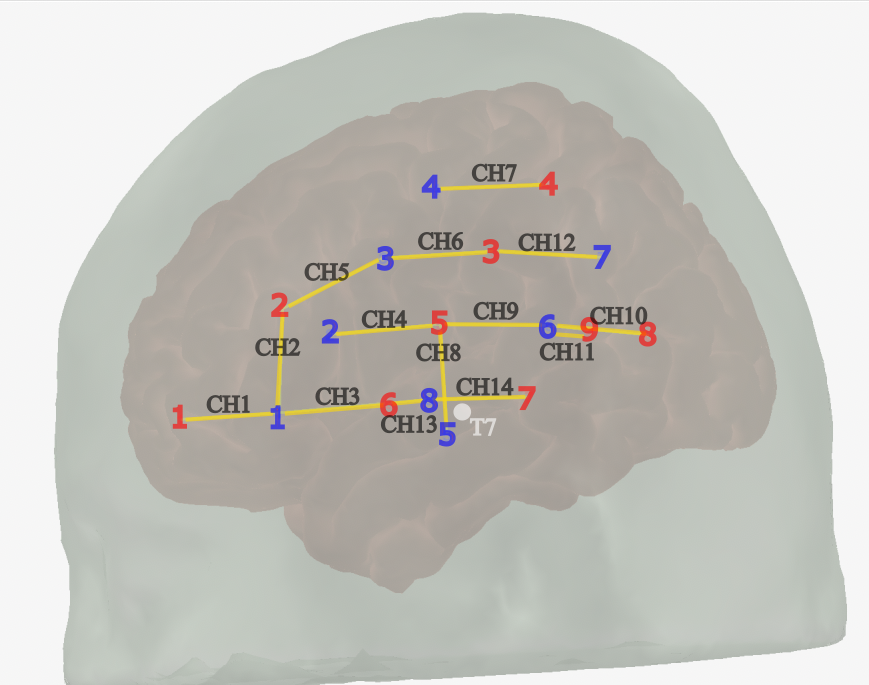
\includegraphics[scale=.48]{bilder/optode_ink.png}
  \caption{Channel Definition}
  \label{fig:somesignal}
\end{figure}

In the following figures. Channels with invalid SCI would not be taken into consideration, and hence would not be shown. Measurements in all channels were plotted in the same scale except for the two short channels marked in thicker outlines. In all our measurements, the changes in the dynamic hemoglobin response were significantly less in the short channels by more than a magnitude.

Our regions of interest (ROI) are defined as the following figure. The auditory cortex is in particular of our interest. Hence, channel 4, channel 8, and channel 9 together formed one region (ROI 2). The rest of the channels formed ROI 1. It is of our interest to compare how the response of the auditory cortex differ from the rest of the left brain hemisphere.

\vspace{1cm}
\begin{figure}[H]
  \centering
    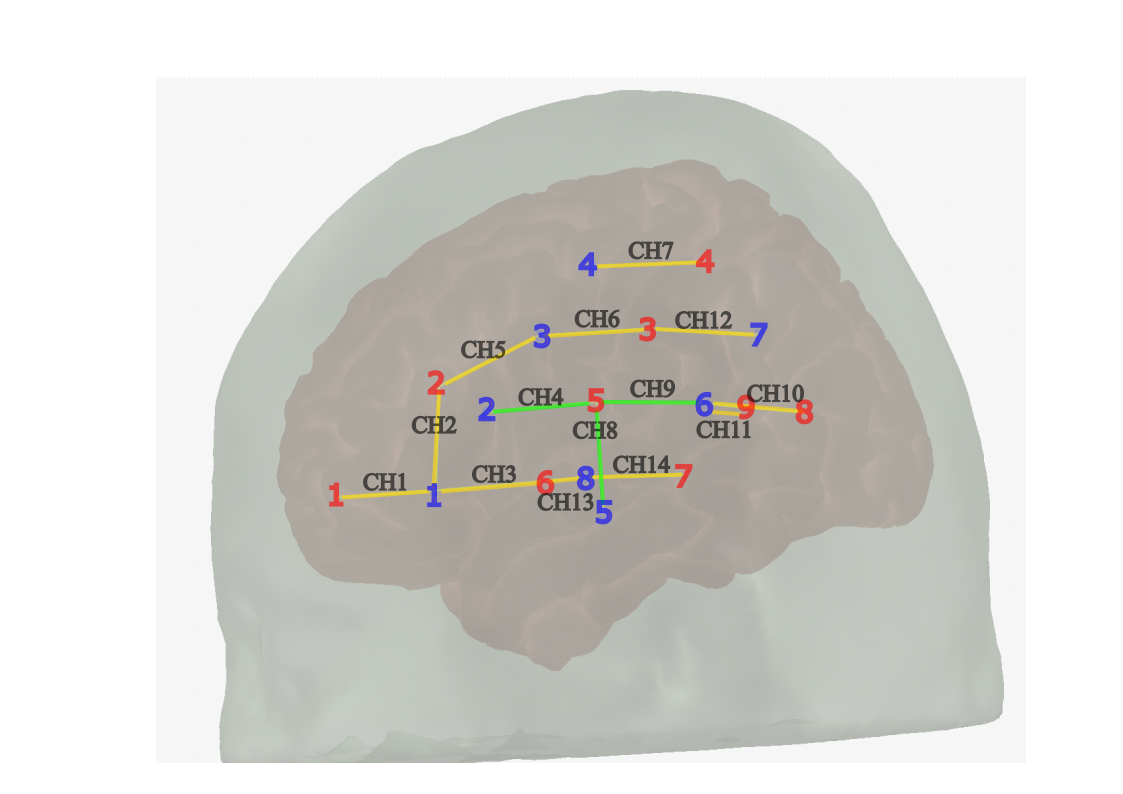
\includegraphics[scale=.5]{bilder/optode_roi_ink.png}
  \caption{ROI Definition}
\end{figure}

\newpage




\section {Participant 3}

\begin{figure}[H]
  \centering
    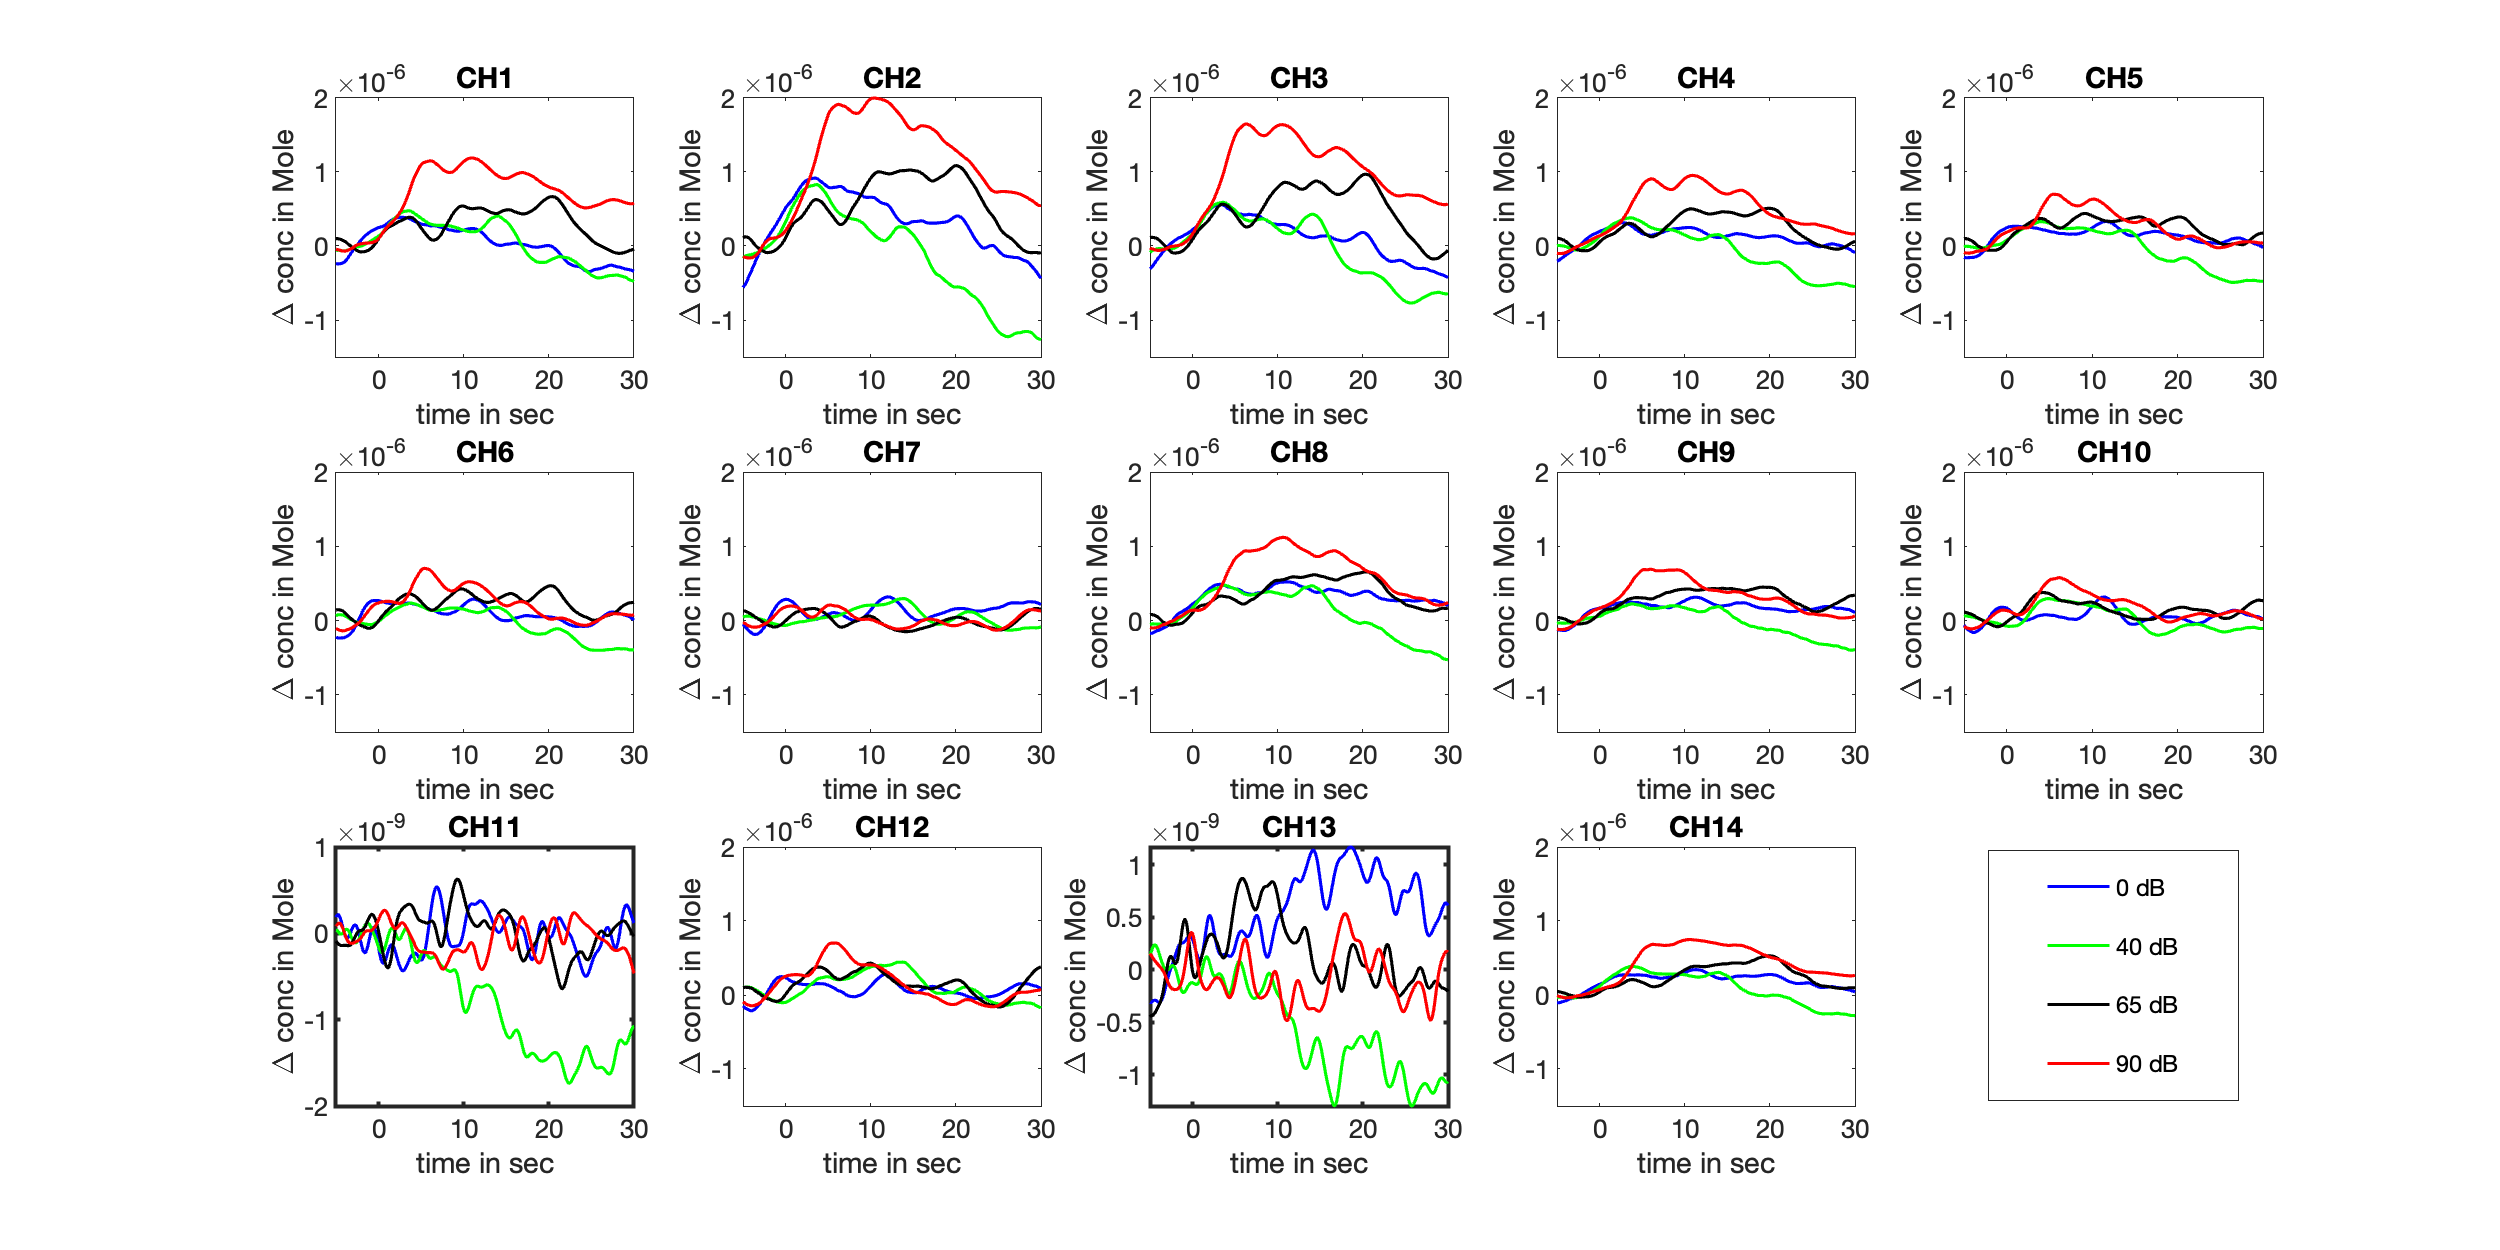
\includegraphics[scale=.4]{bilder/HbO_Mole/sub_jonas_s_HbO.png}
  \caption{Measurement from participant 3.}
  \label{fig:somesignal}
\end{figure}

\begin{figure}[H]
  \centering
    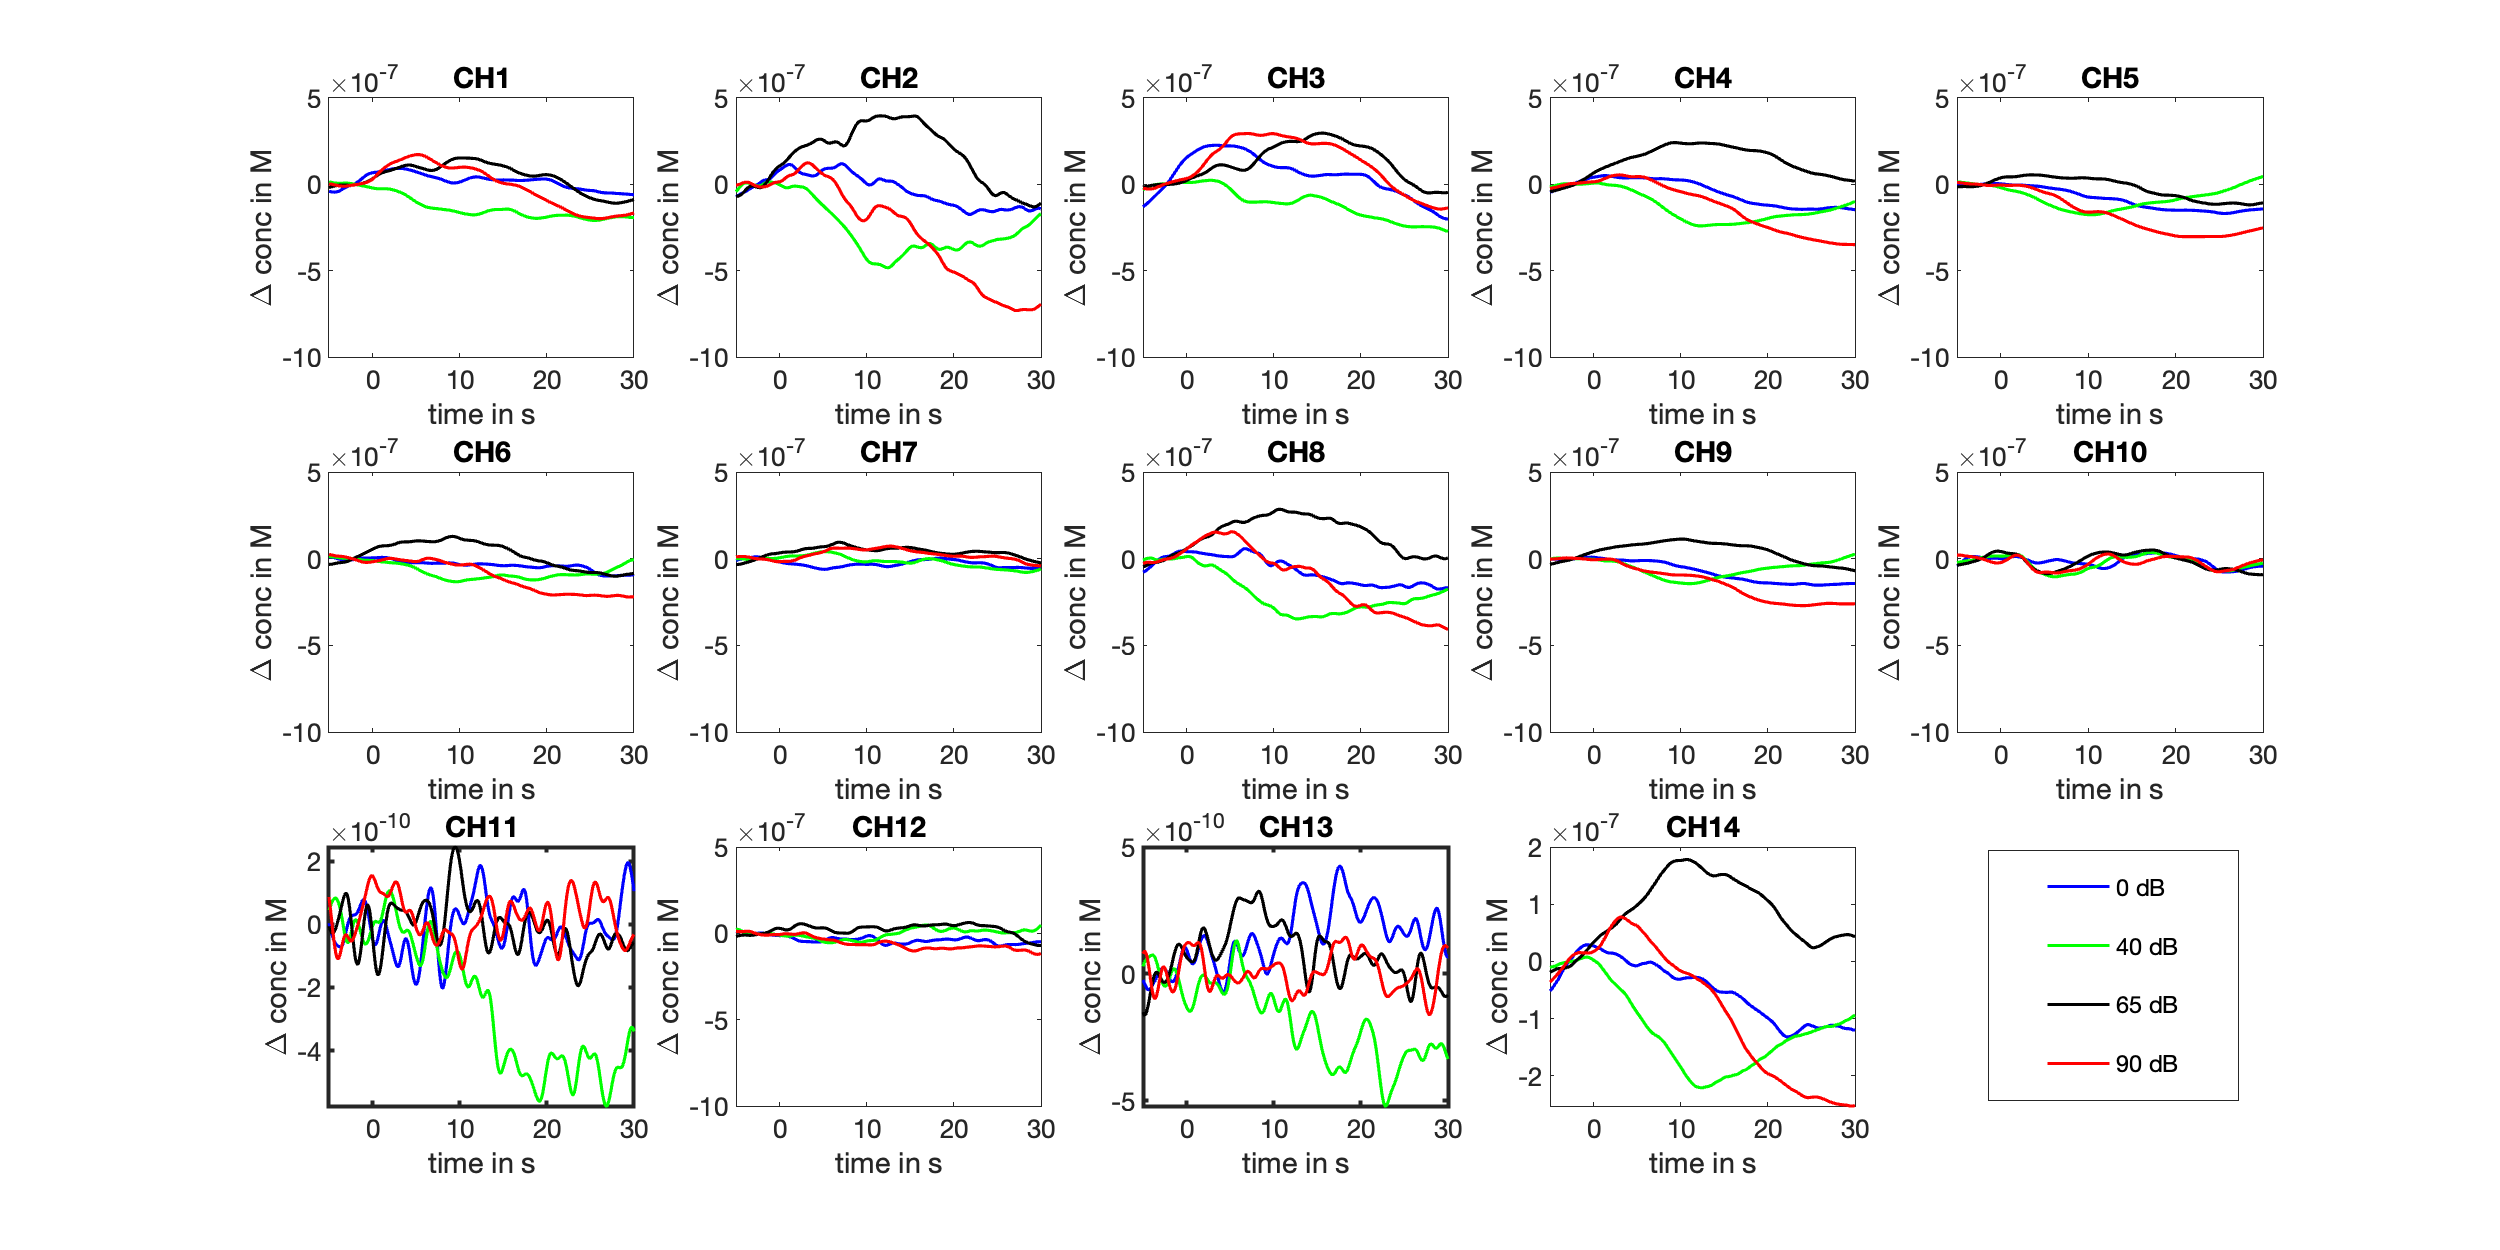
\includegraphics[scale=.4]{bilder/HbR_Mole/sub_jonas_s_HbR.png}
  \caption{Measurement from participant 3.}
  \label{fig:somesignal}
\end{figure}

\begin{figure}[H]
  \centering
    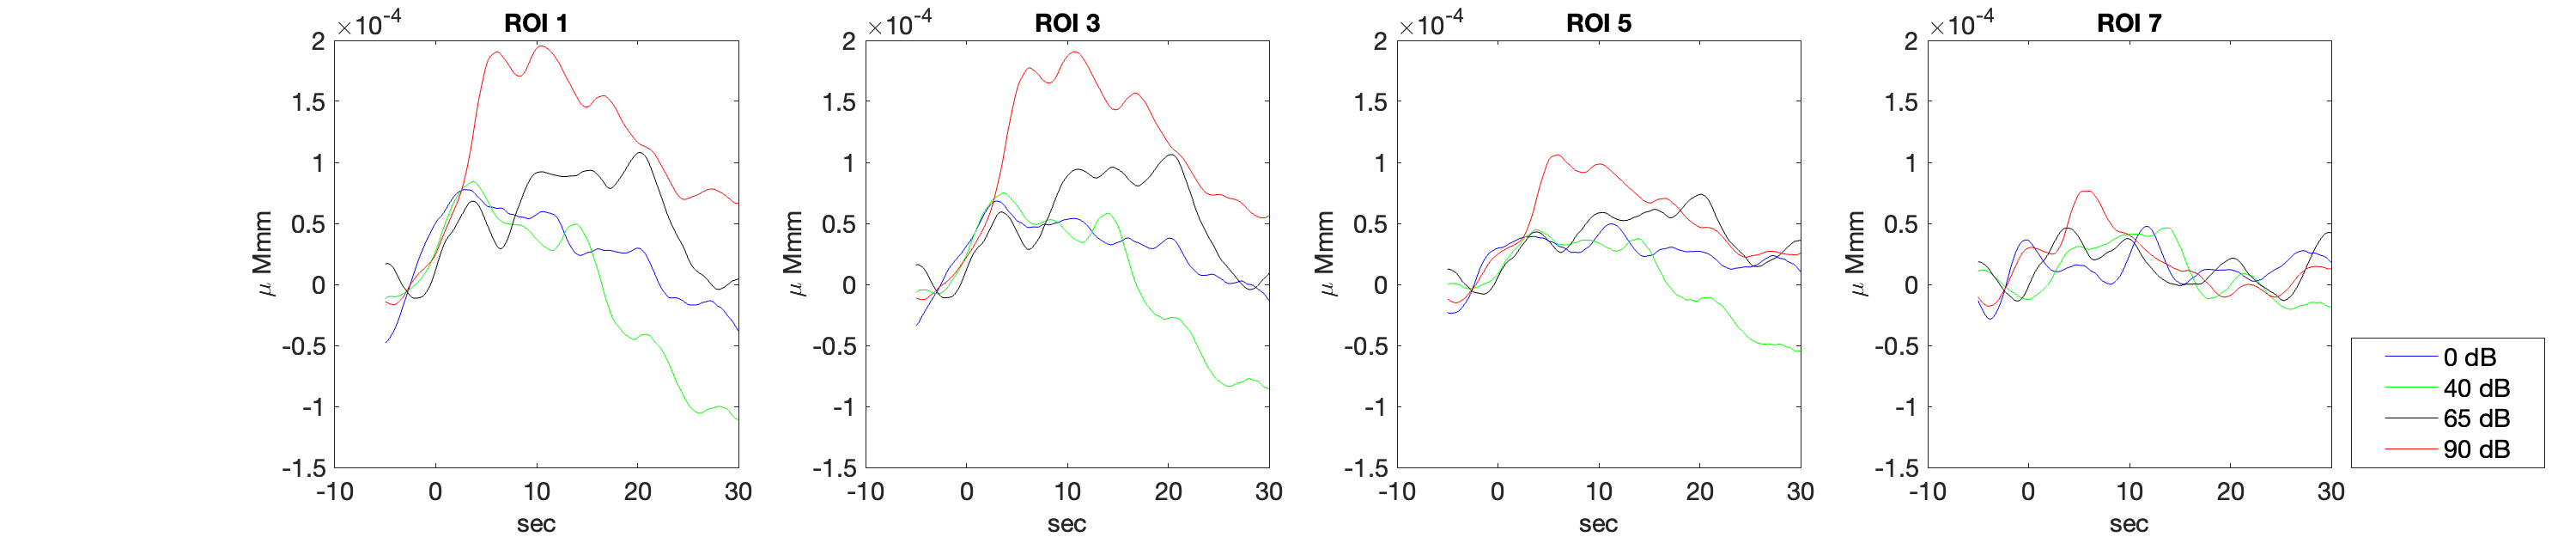
\includegraphics[scale=.3]{bilder/ROI/sub_jonas_s_HbO.png}
  \caption{Measurement from participant  3.}
\end{figure}

The results from this participant was the closest one to the results reported by Weder et al. For the oxygenated hemoglobin HbO waveform morphology, tonic response could be observed in channel 1, 2, and 3, and phasic response could be observed in channel 10 and 12.

\newpage





\section {Participant 5}
\begin{figure}[H]
  \centering
    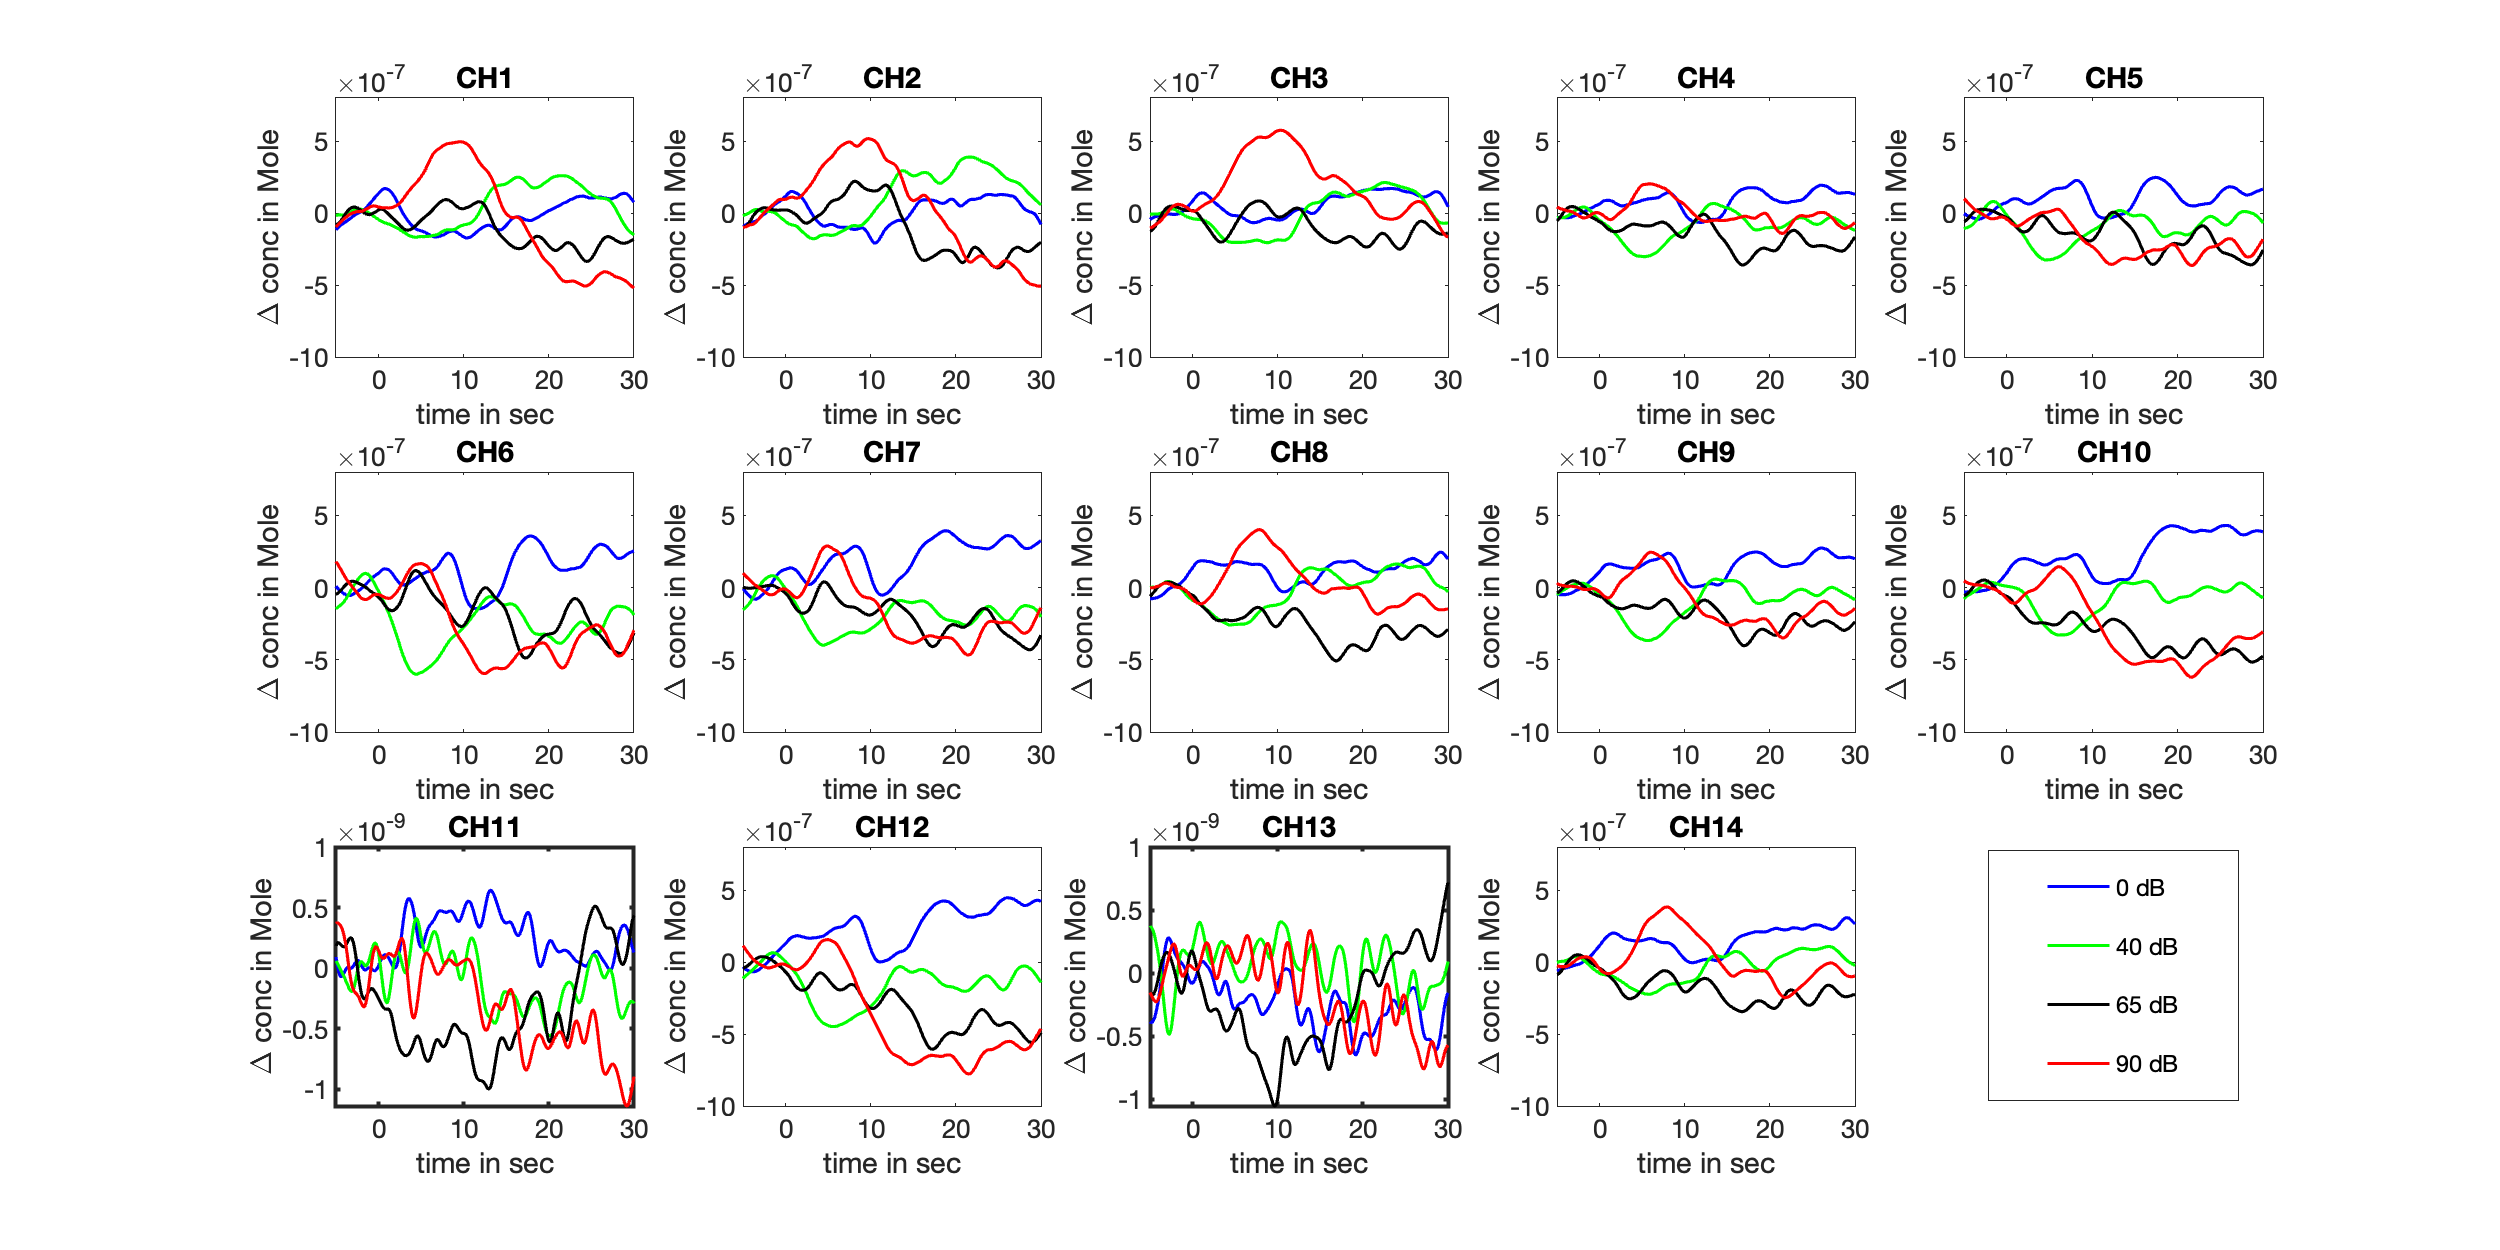
\includegraphics[scale=.4]{bilder/HbO_Mole/sub_lukas_s_HbO.png}
  \caption{Measurement from participant 5.}
  \label{fig:somesignal}
\end{figure}

\begin{figure}[H]
  \centering
    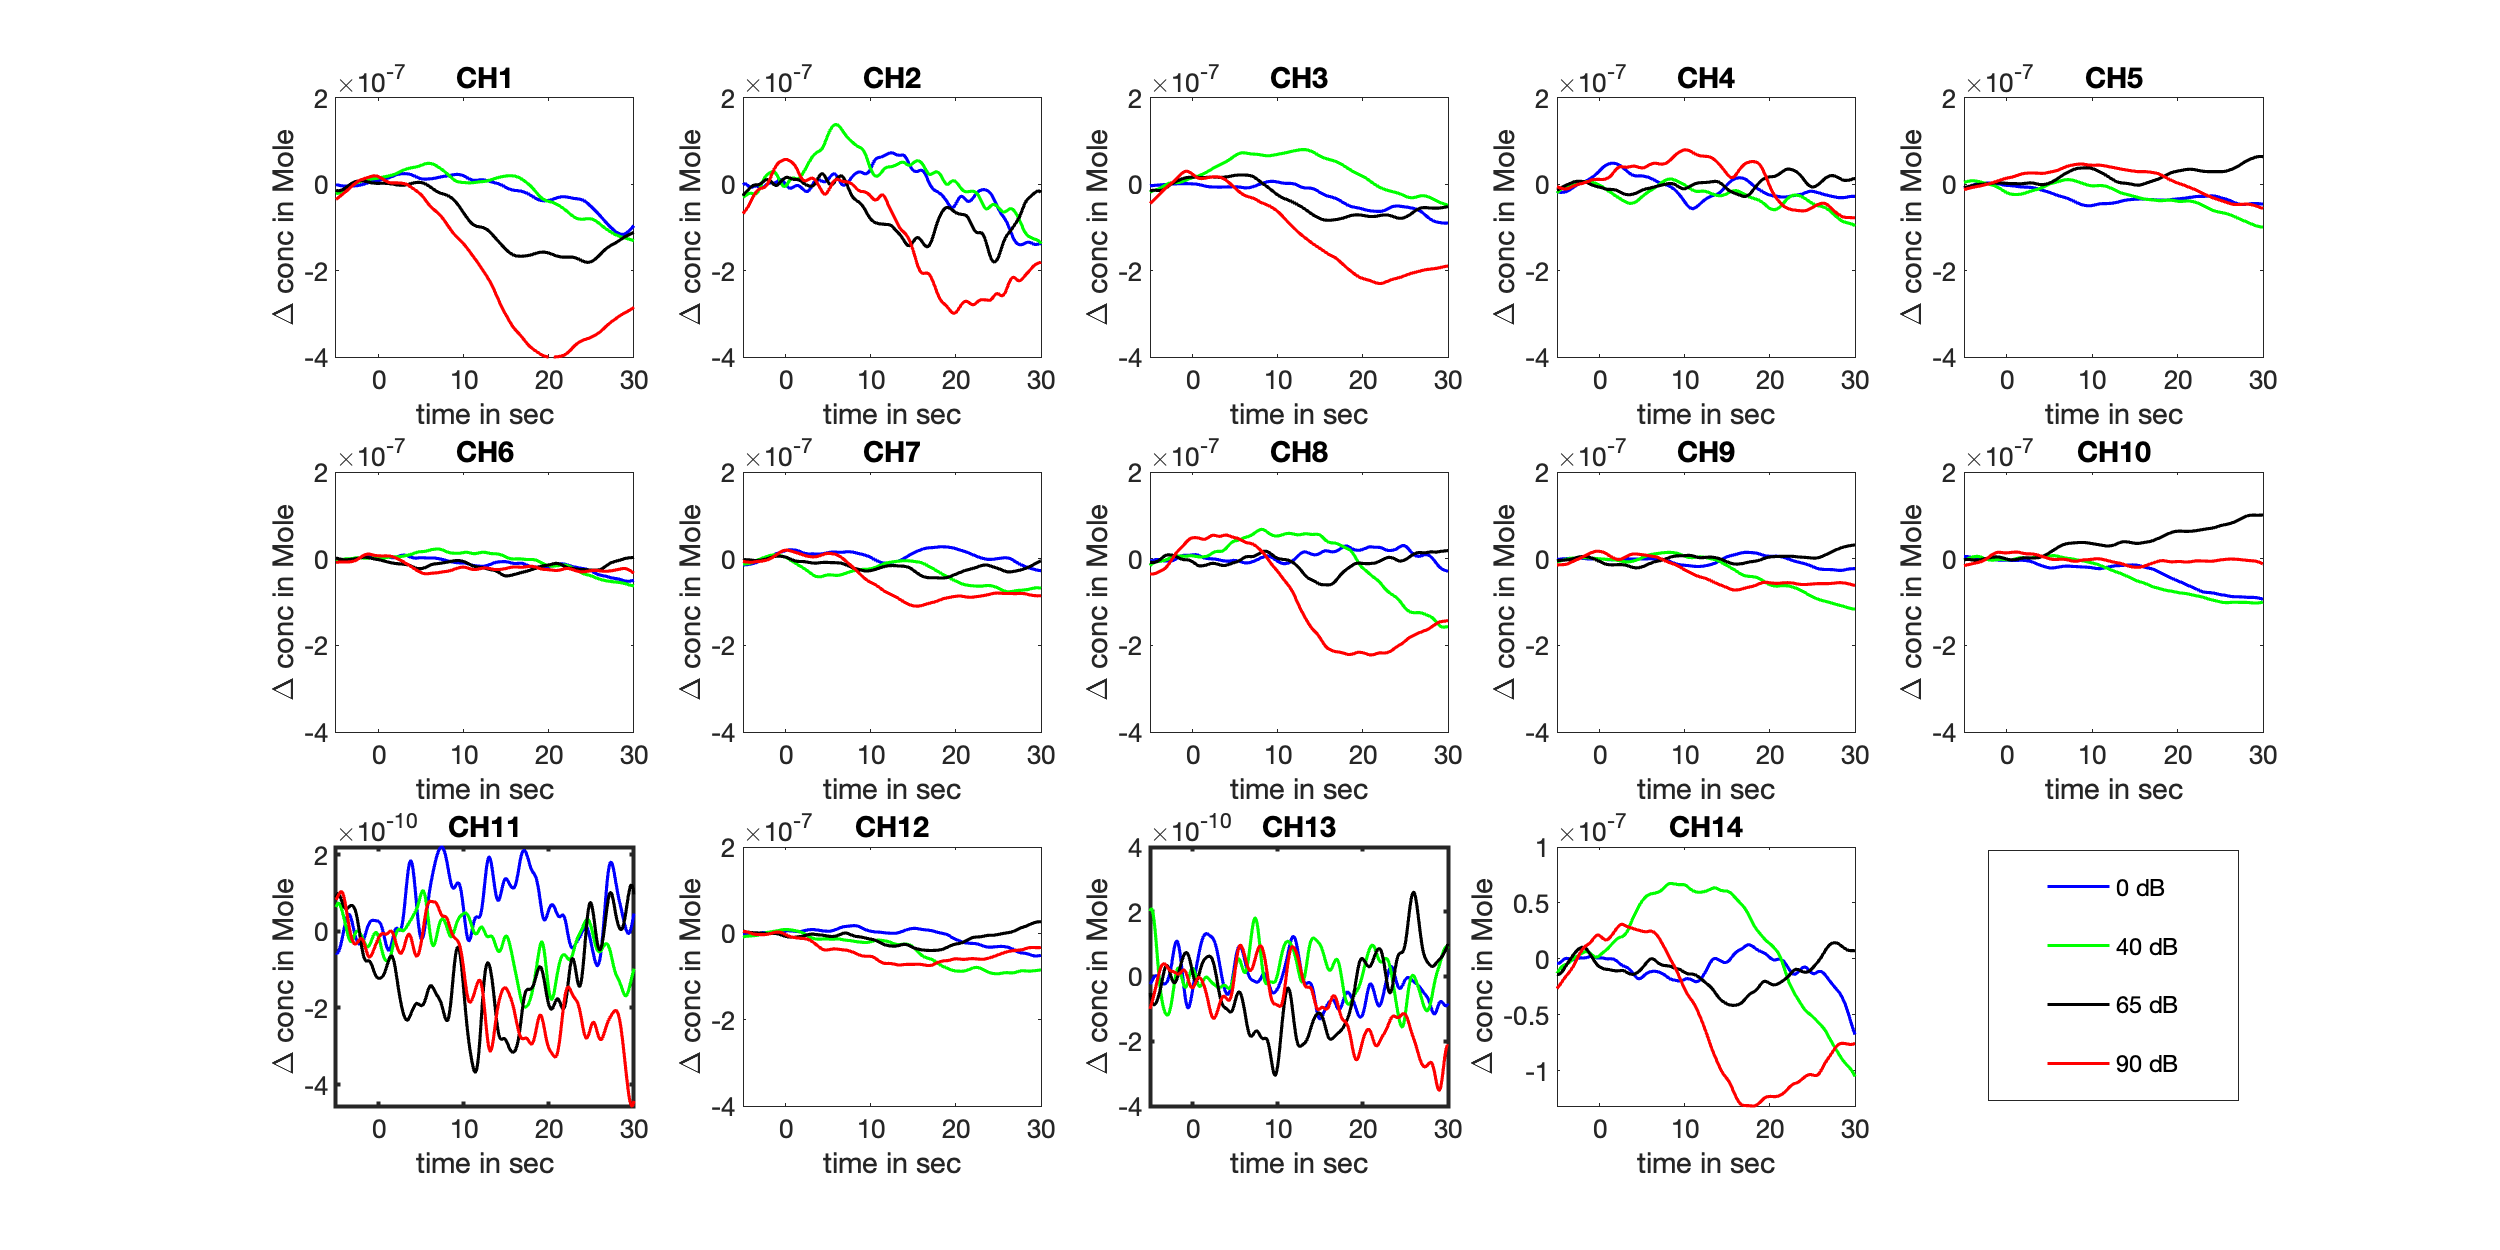
\includegraphics[scale=.4]{bilder/HbR_Mole/sub_lukas_s_HbR.png}
  \caption{Measurement from participant 5.}
  \label{fig:somesignal}
\end{figure}

\begin{figure}[H]
  \centering
    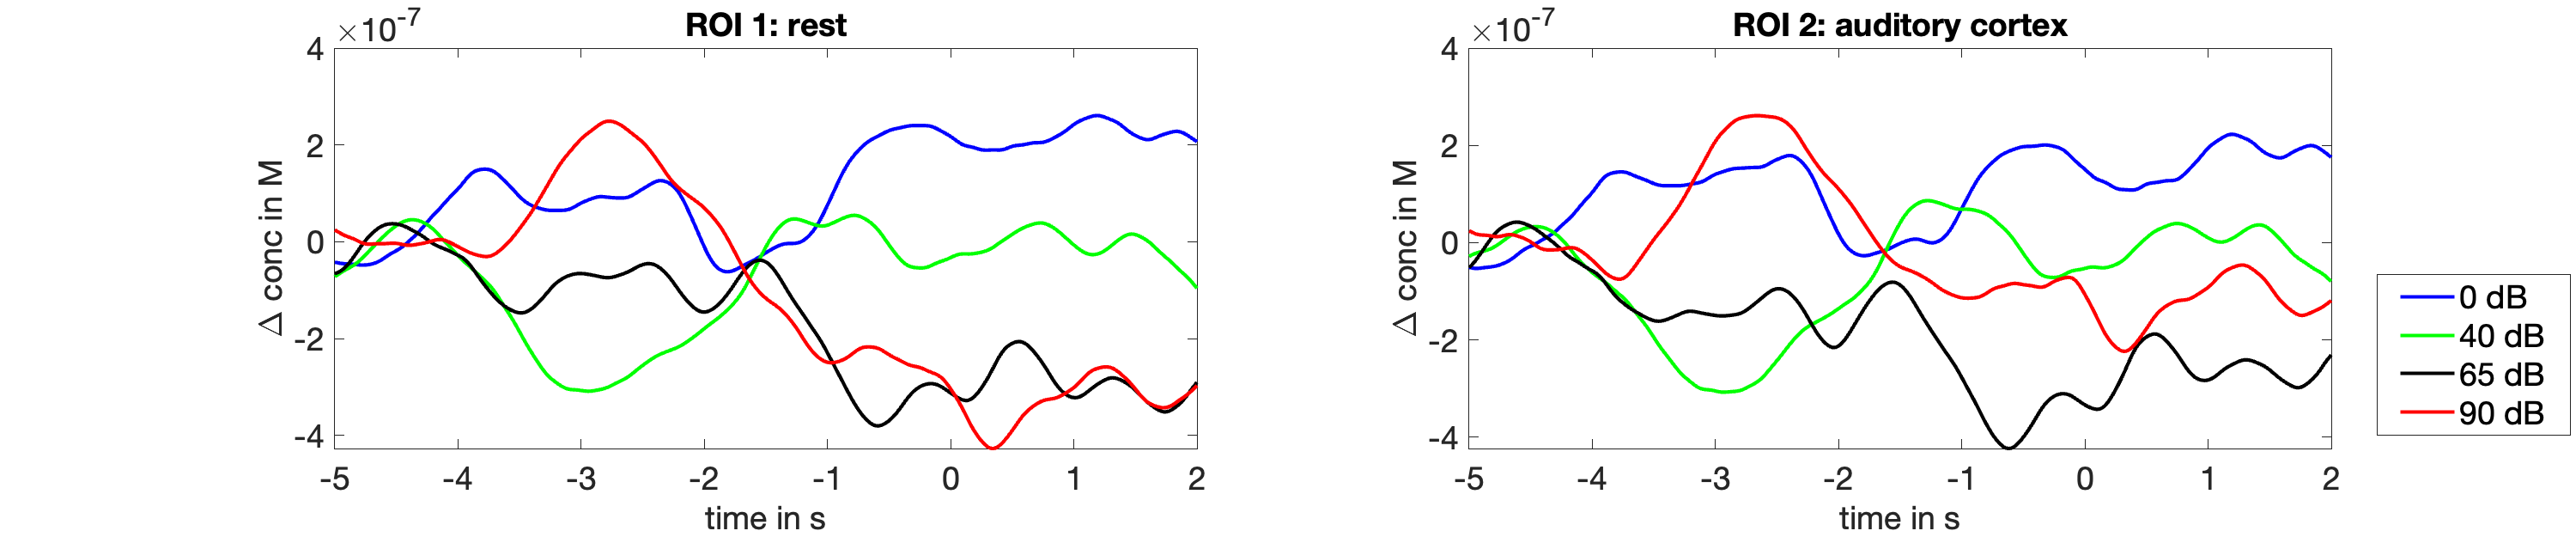
\includegraphics[scale=.29]{bilder/ROI/sub_lukas_s_HbO.png}
  \caption{Measurement from participant 5.}
\end{figure}

For the \acrlong{HbO} (\acrshort{HbO} ) waveform, there were significantly larger on-sets for the 90 dB sound stimuli in Channel 1, 2, and 3, i.e. around the Broca's area.

Apart from this, the waveforms for \acrlong{HbR} (\acrshort{HbR}), were also quite different from the ones Weder et al \citeyear{Weder2018}. reported. For the loudest sound stimuli, channels overlying the caudal superior temporal gyrus and channels over Broca's area showed clear phasic response. 


\newpage




\section {Participant 6}
\begin{figure}[H]
  \centering
    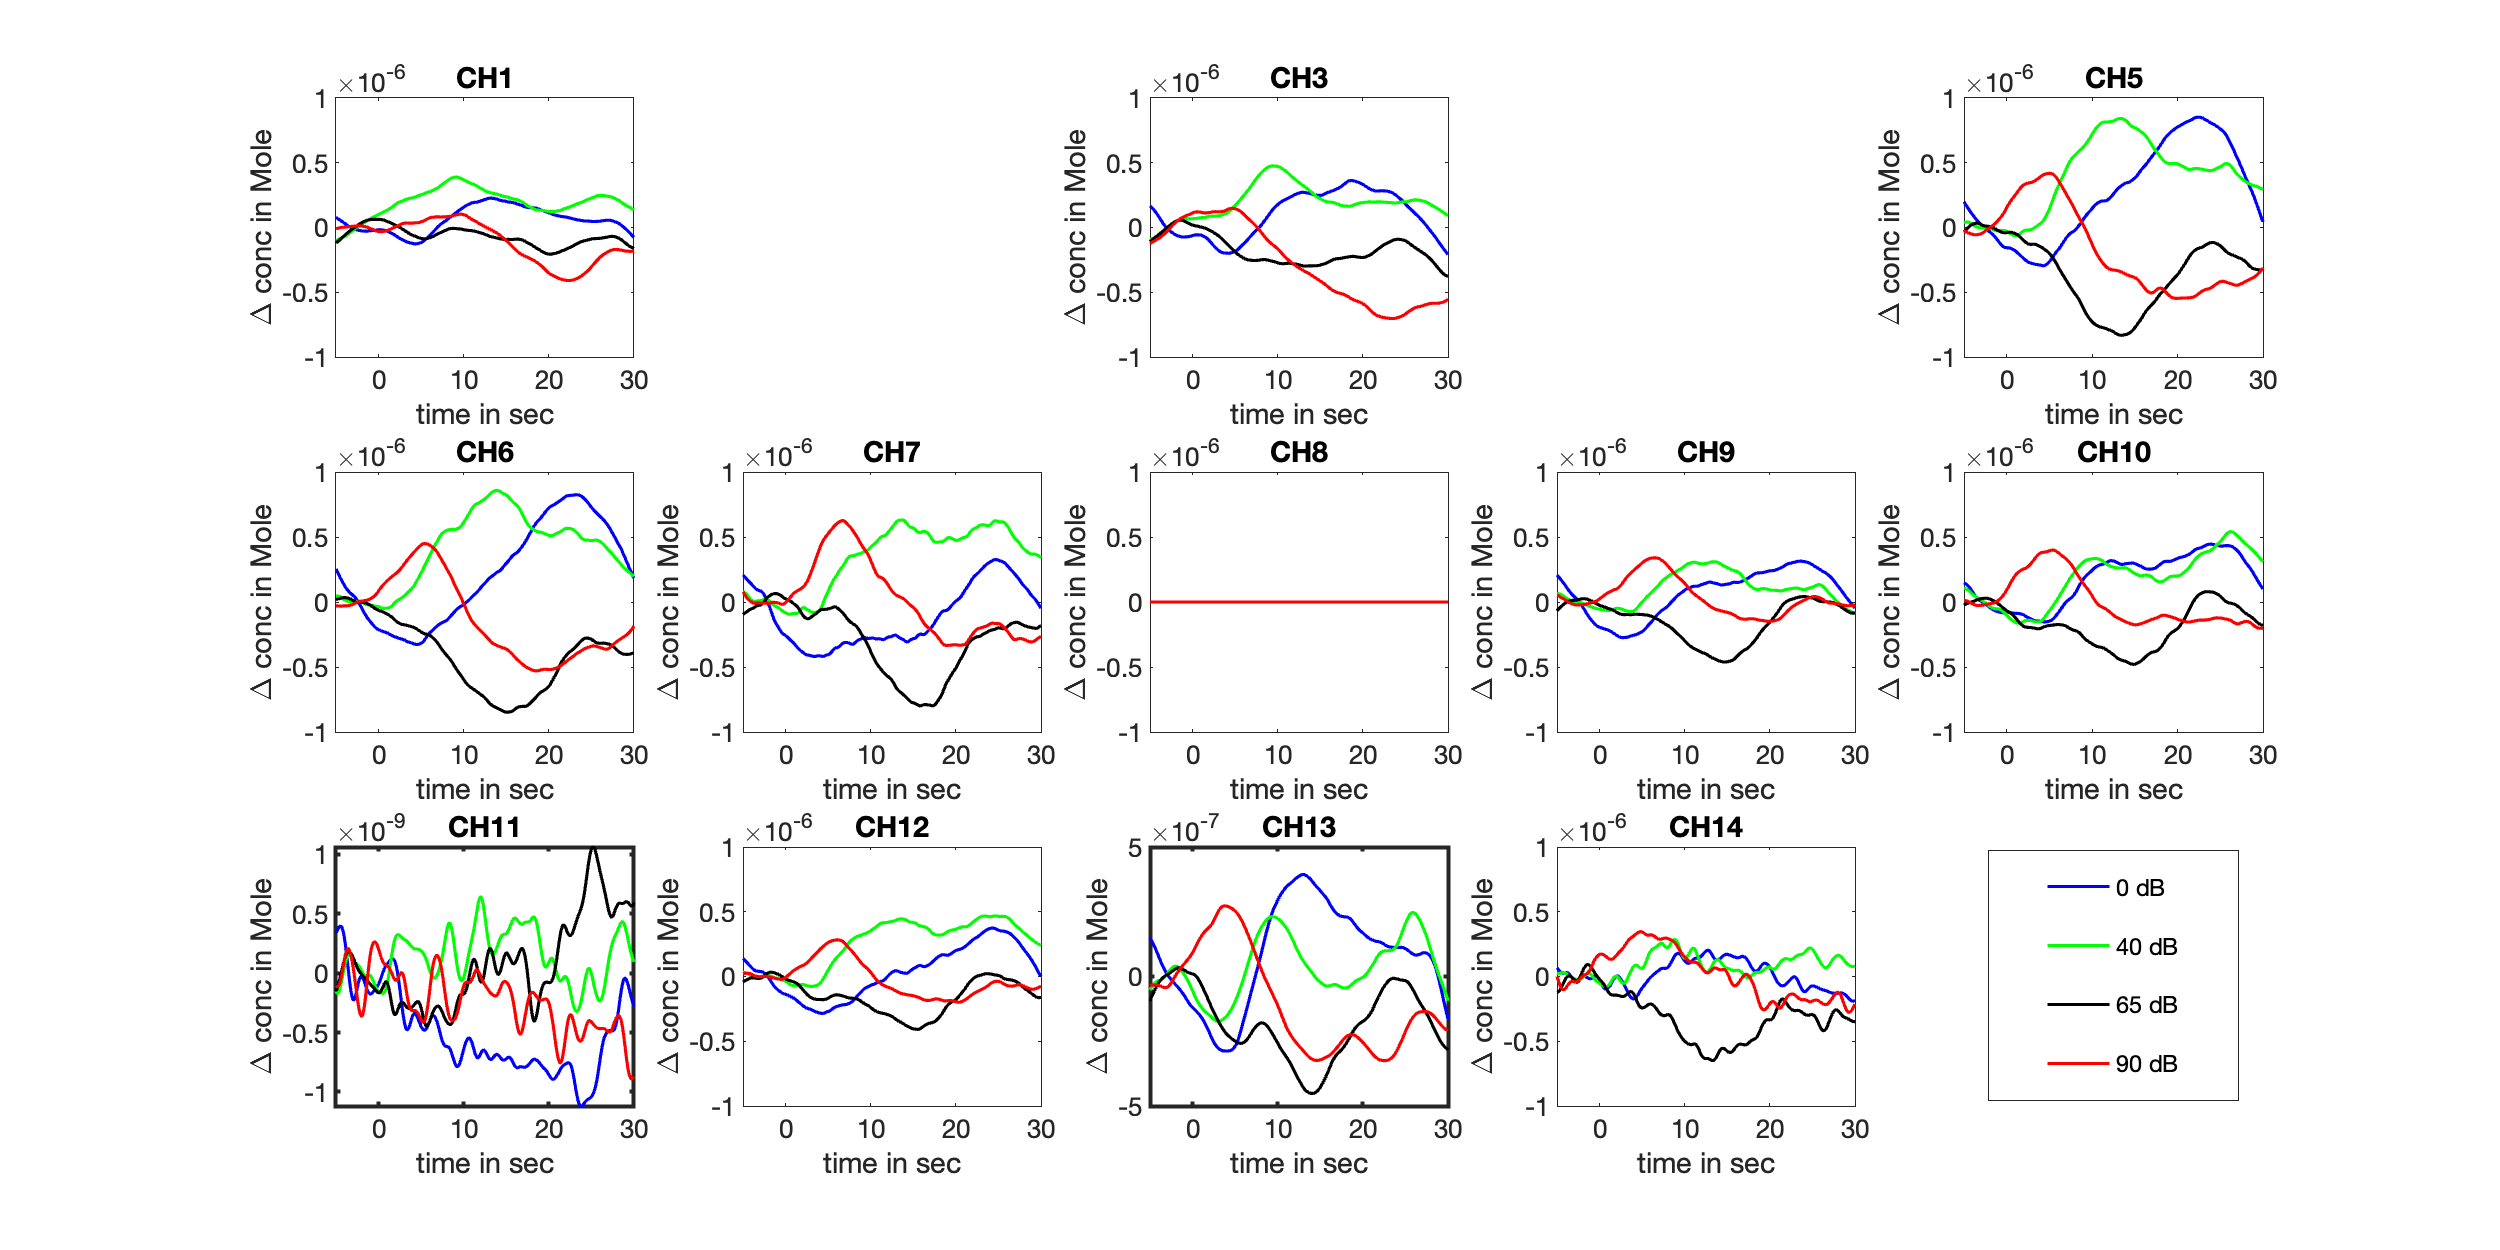
\includegraphics[scale=.4]{bilder/HbO_Mole/sub_shelia_s_HbO.png}
  \caption{Measurement from participant 6.}
  \label{fig:somesignal}
\end{figure}

\begin{figure}[H]
  \centering
    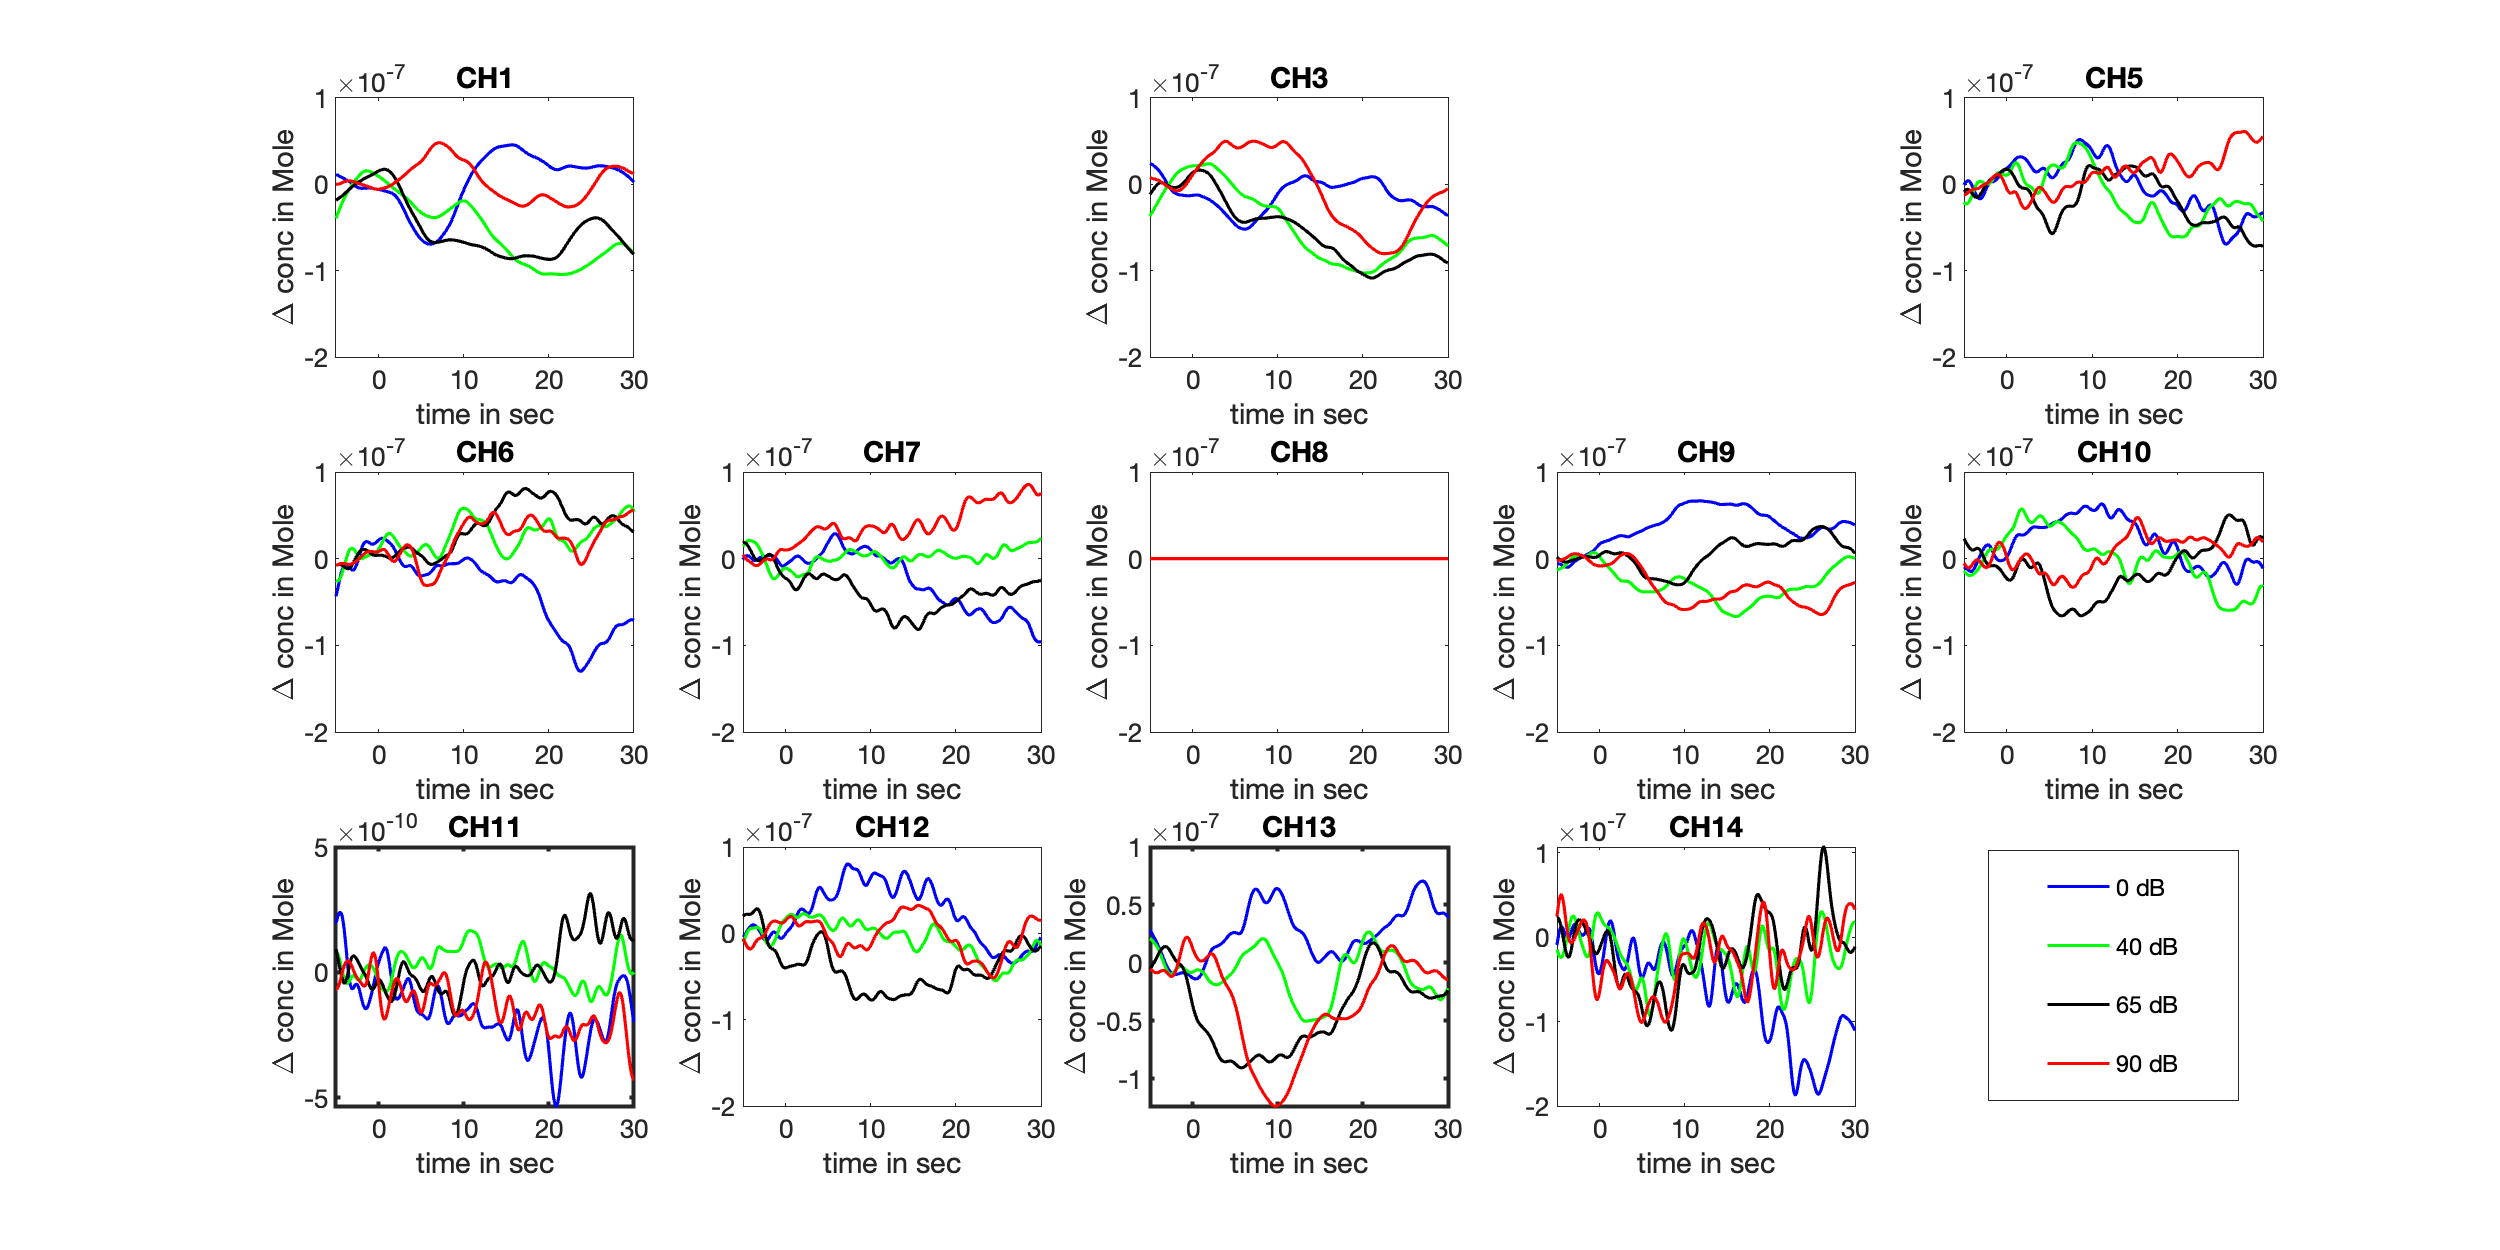
\includegraphics[scale=.4]{bilder/HbR_Mole/sub_shelia_s_HbR.png}
  \caption{Measurement from participant 6.}
  \label{fig:somesignal}
\end{figure}

\begin{figure}[H]
  \centering
    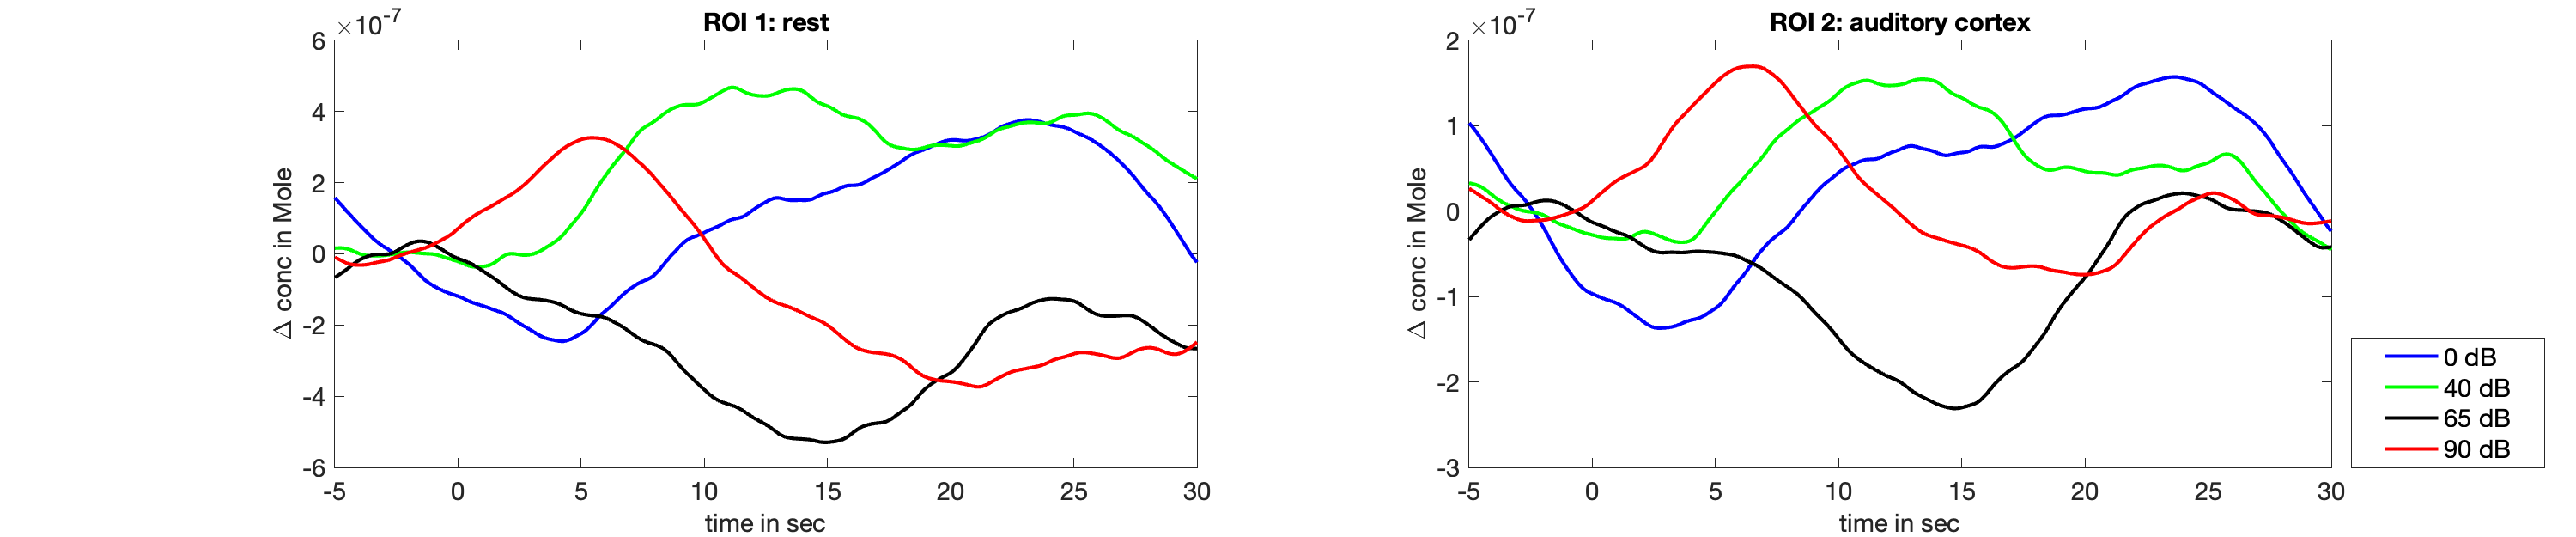
\includegraphics[scale=.29]{bilder/ROI/sub_shelia_s_HbO.png}
  \caption{Measurement from participant  6.}
\end{figure}

For the oxygenated hemoglobin, \acrshort{HbO} waveform, the loudest sound stimuli resulted in phasic response for almost all the channels. In addition, it also resulted in faster on-set compared with other stimuli of lower sound pressure levels.

On the other hand, as for the deoxygenated hemoglobin, \acrshort{HbR} response, results from multiple channels appeared to be noisy even if the SCI values were already above the suggested threshold.

\newpage





\section {Participant 7}
\begin{figure}[H]
  \centering
    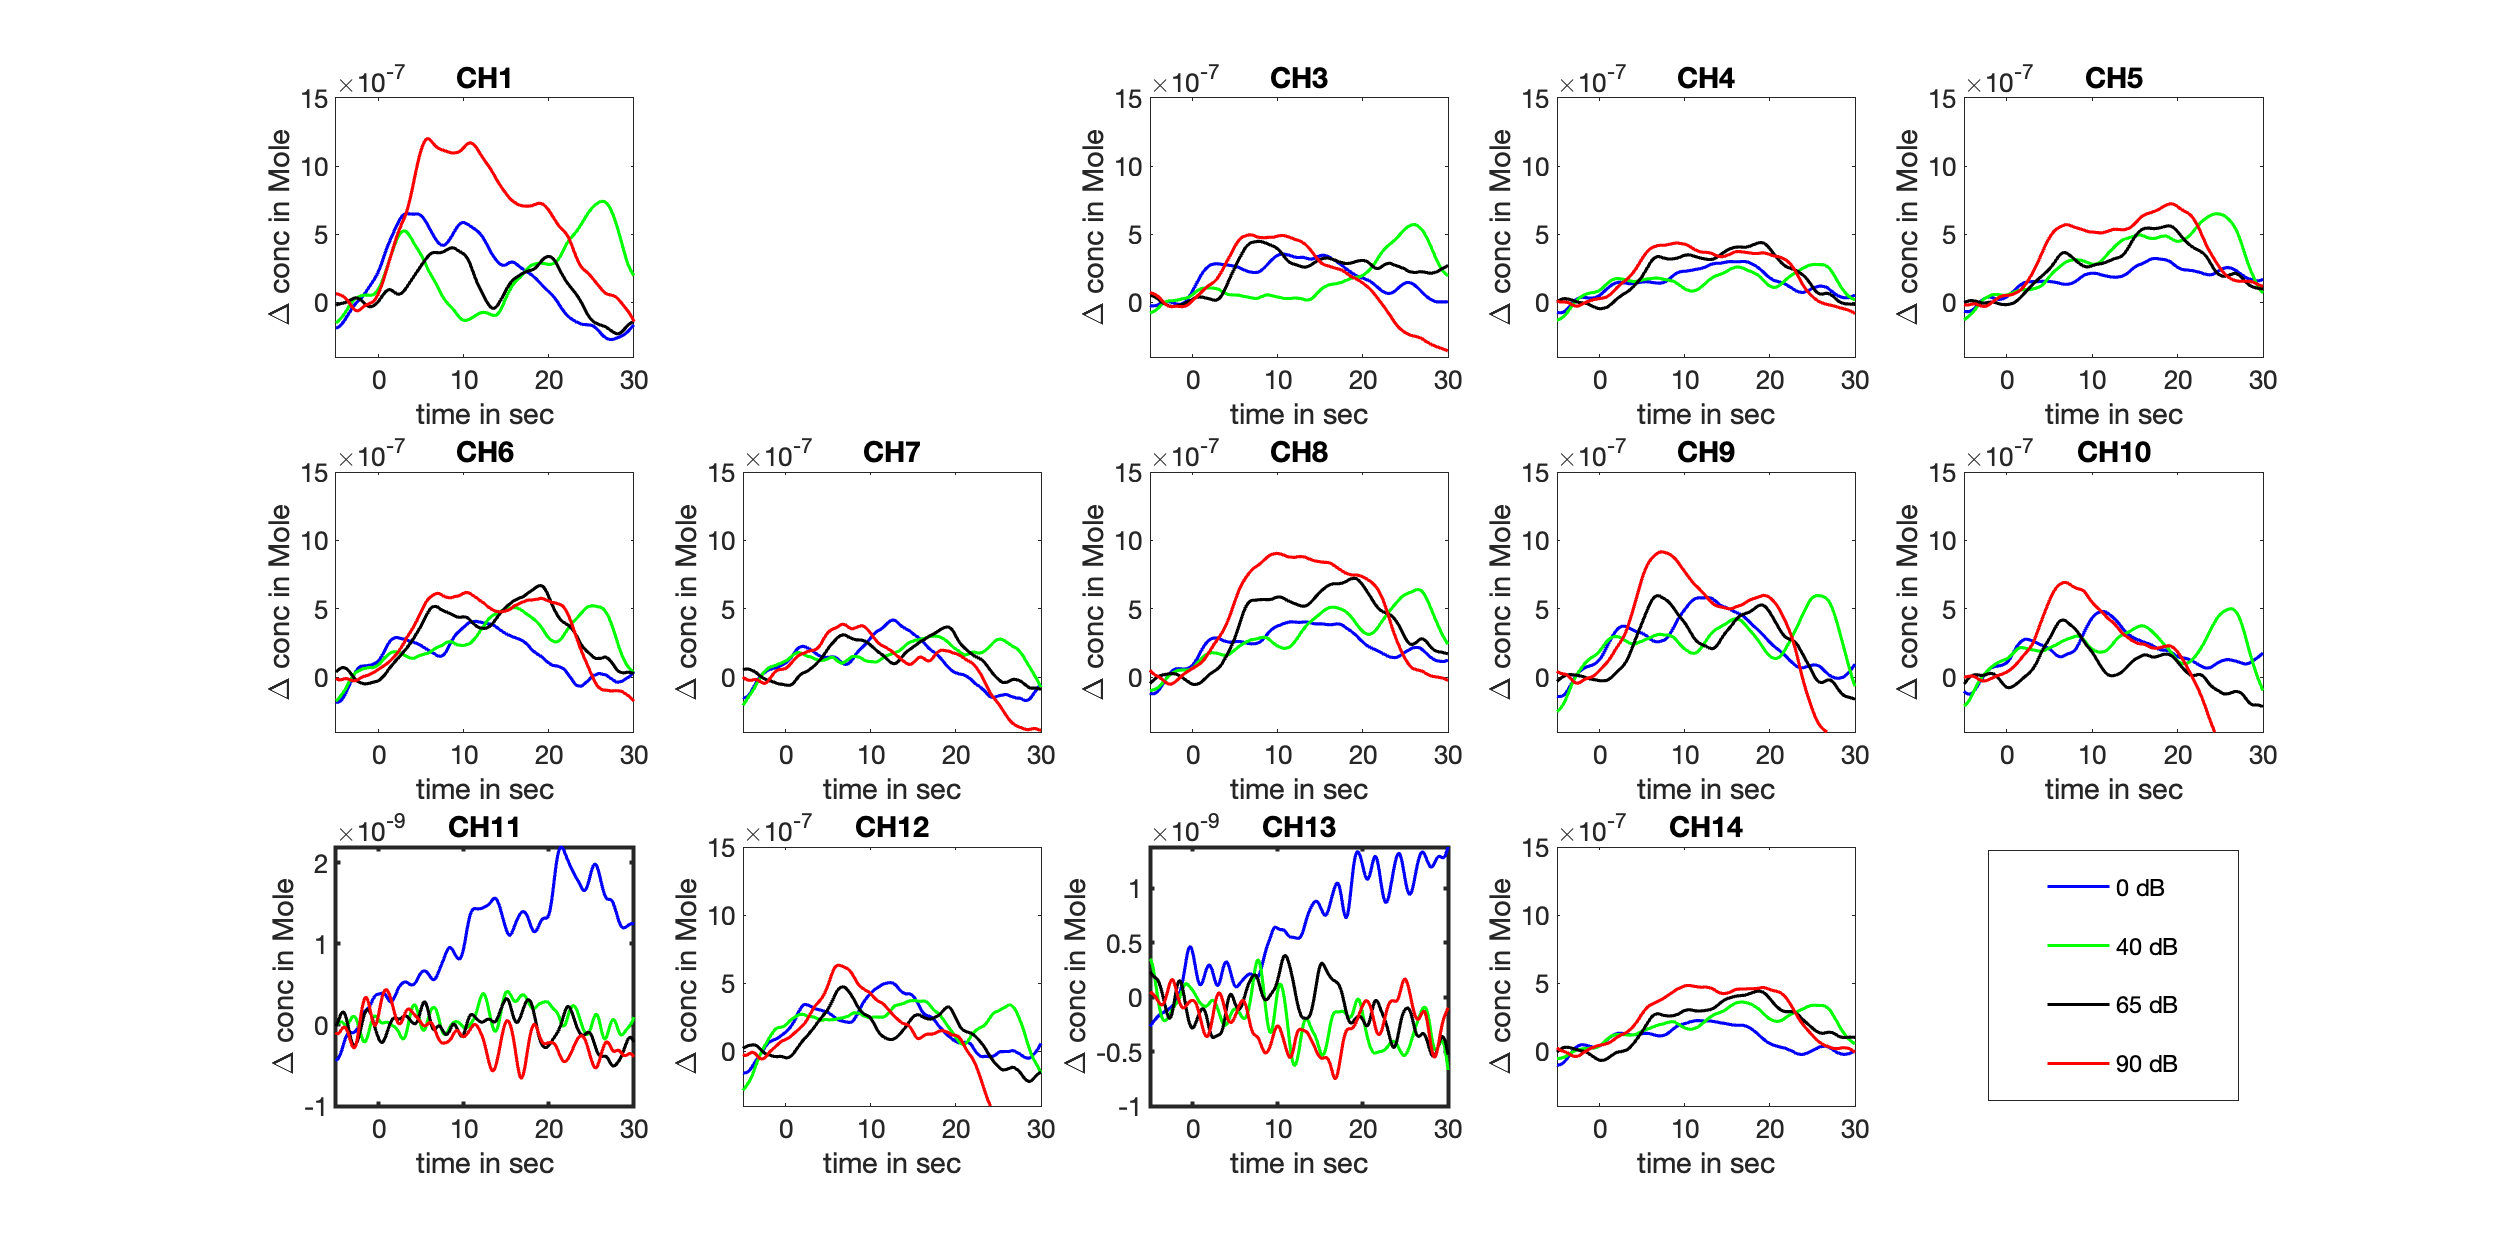
\includegraphics[scale=.4]{bilder/HbO_Mole/sub_liao_s_HbO.png}
  \caption{Measurement from participant 7.}
  \label{fig:somesignal}
\end{figure}

\begin{figure}[H]
  \centering
    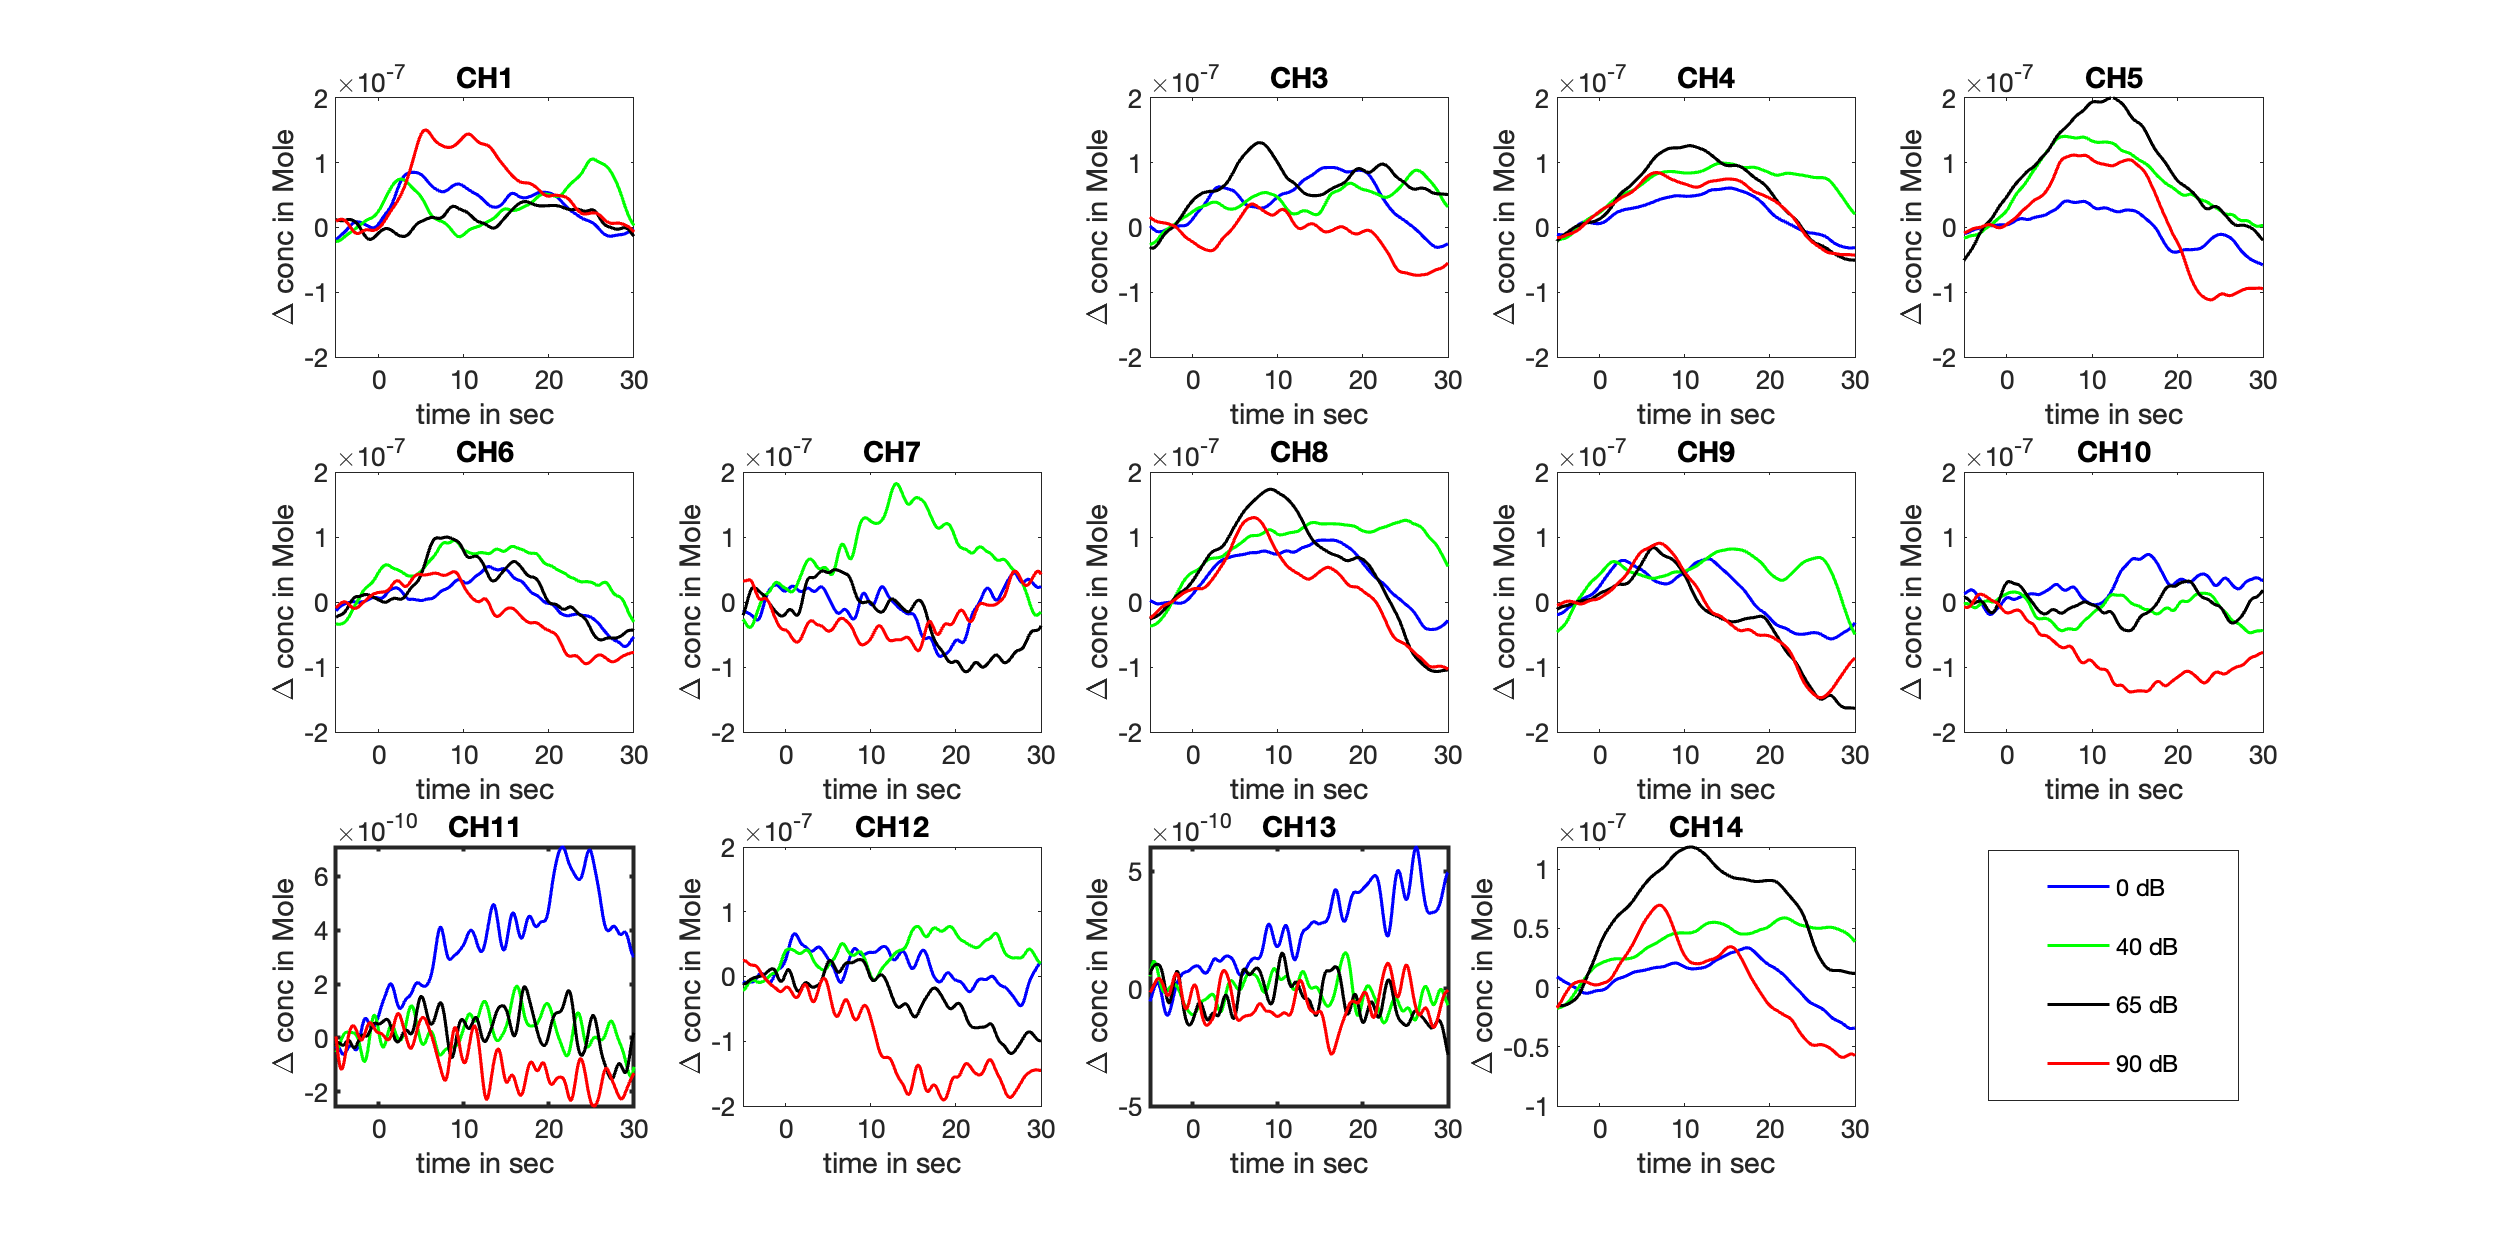
\includegraphics[scale=.4]{bilder/HbR_Mole/sub_liao_s_HbR.png}
  \caption{Measurement from participant 7.}
  \label{fig:somesignal}
\end{figure}

\begin{figure}[H]
  \centering
    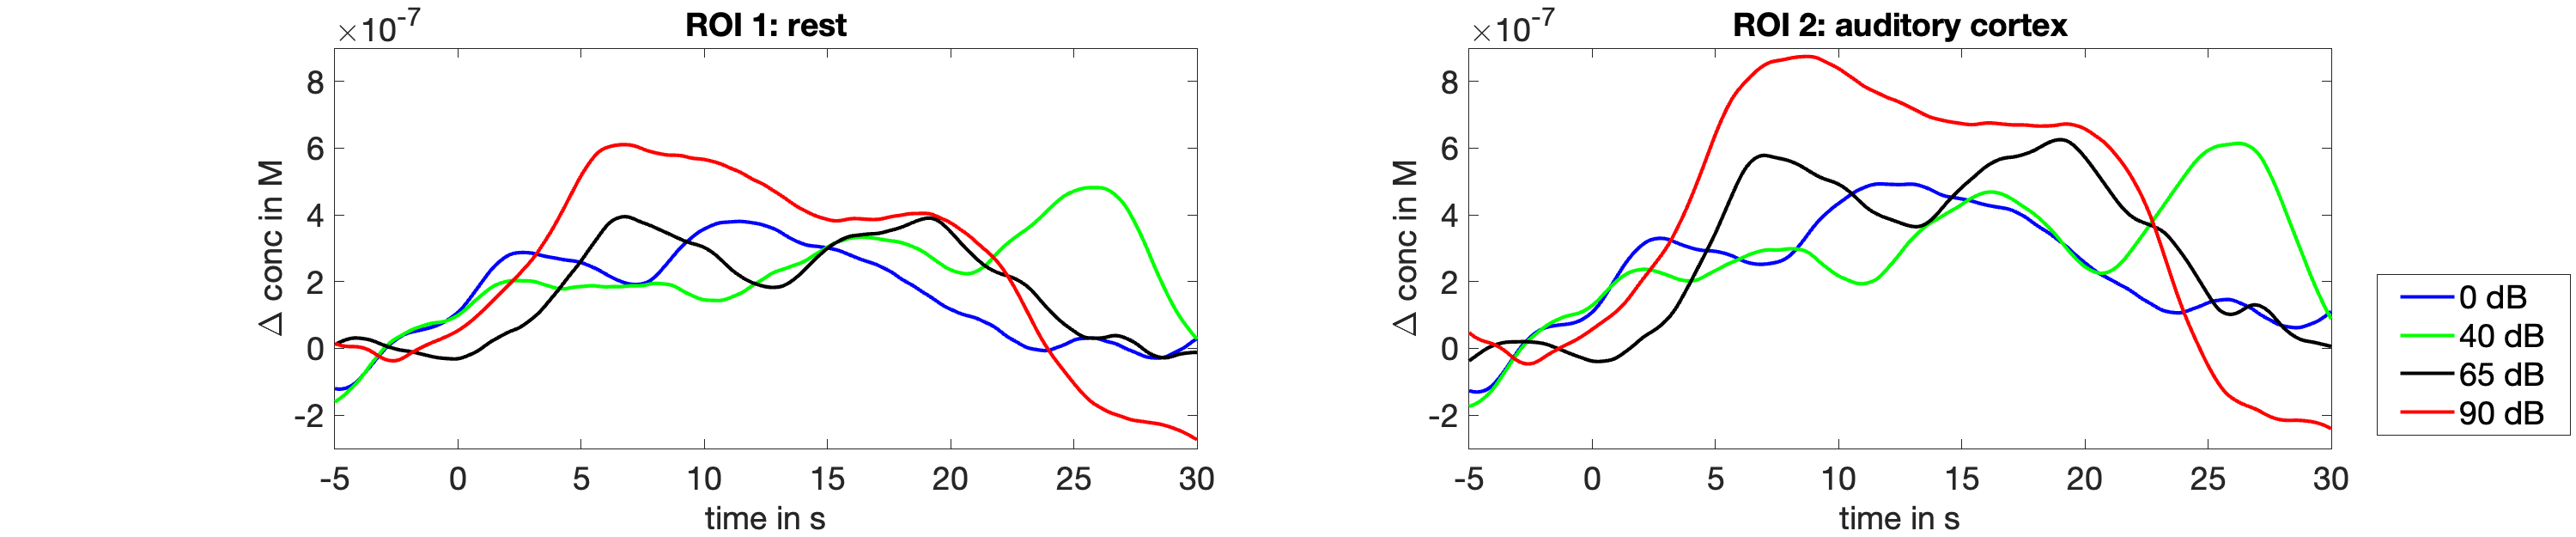
\includegraphics[scale=.29]{bilder/ROI/sub_liao_s_HbO.png}
  \caption{Measurement from participant 7.}
\end{figure}

The results from this participant are rather indeterminant to differentiate between response to different sound pressure levels.

\newpage



\section {Participant 4}
There were also some poor measurements even though the SCI is above the threshold 0.75. For example, in our case of participant 4. One possible reason can be due to the thick dark hair of the participant. Light absorption can affect the result greatly.

\begin{figure}[H]
  \centering
    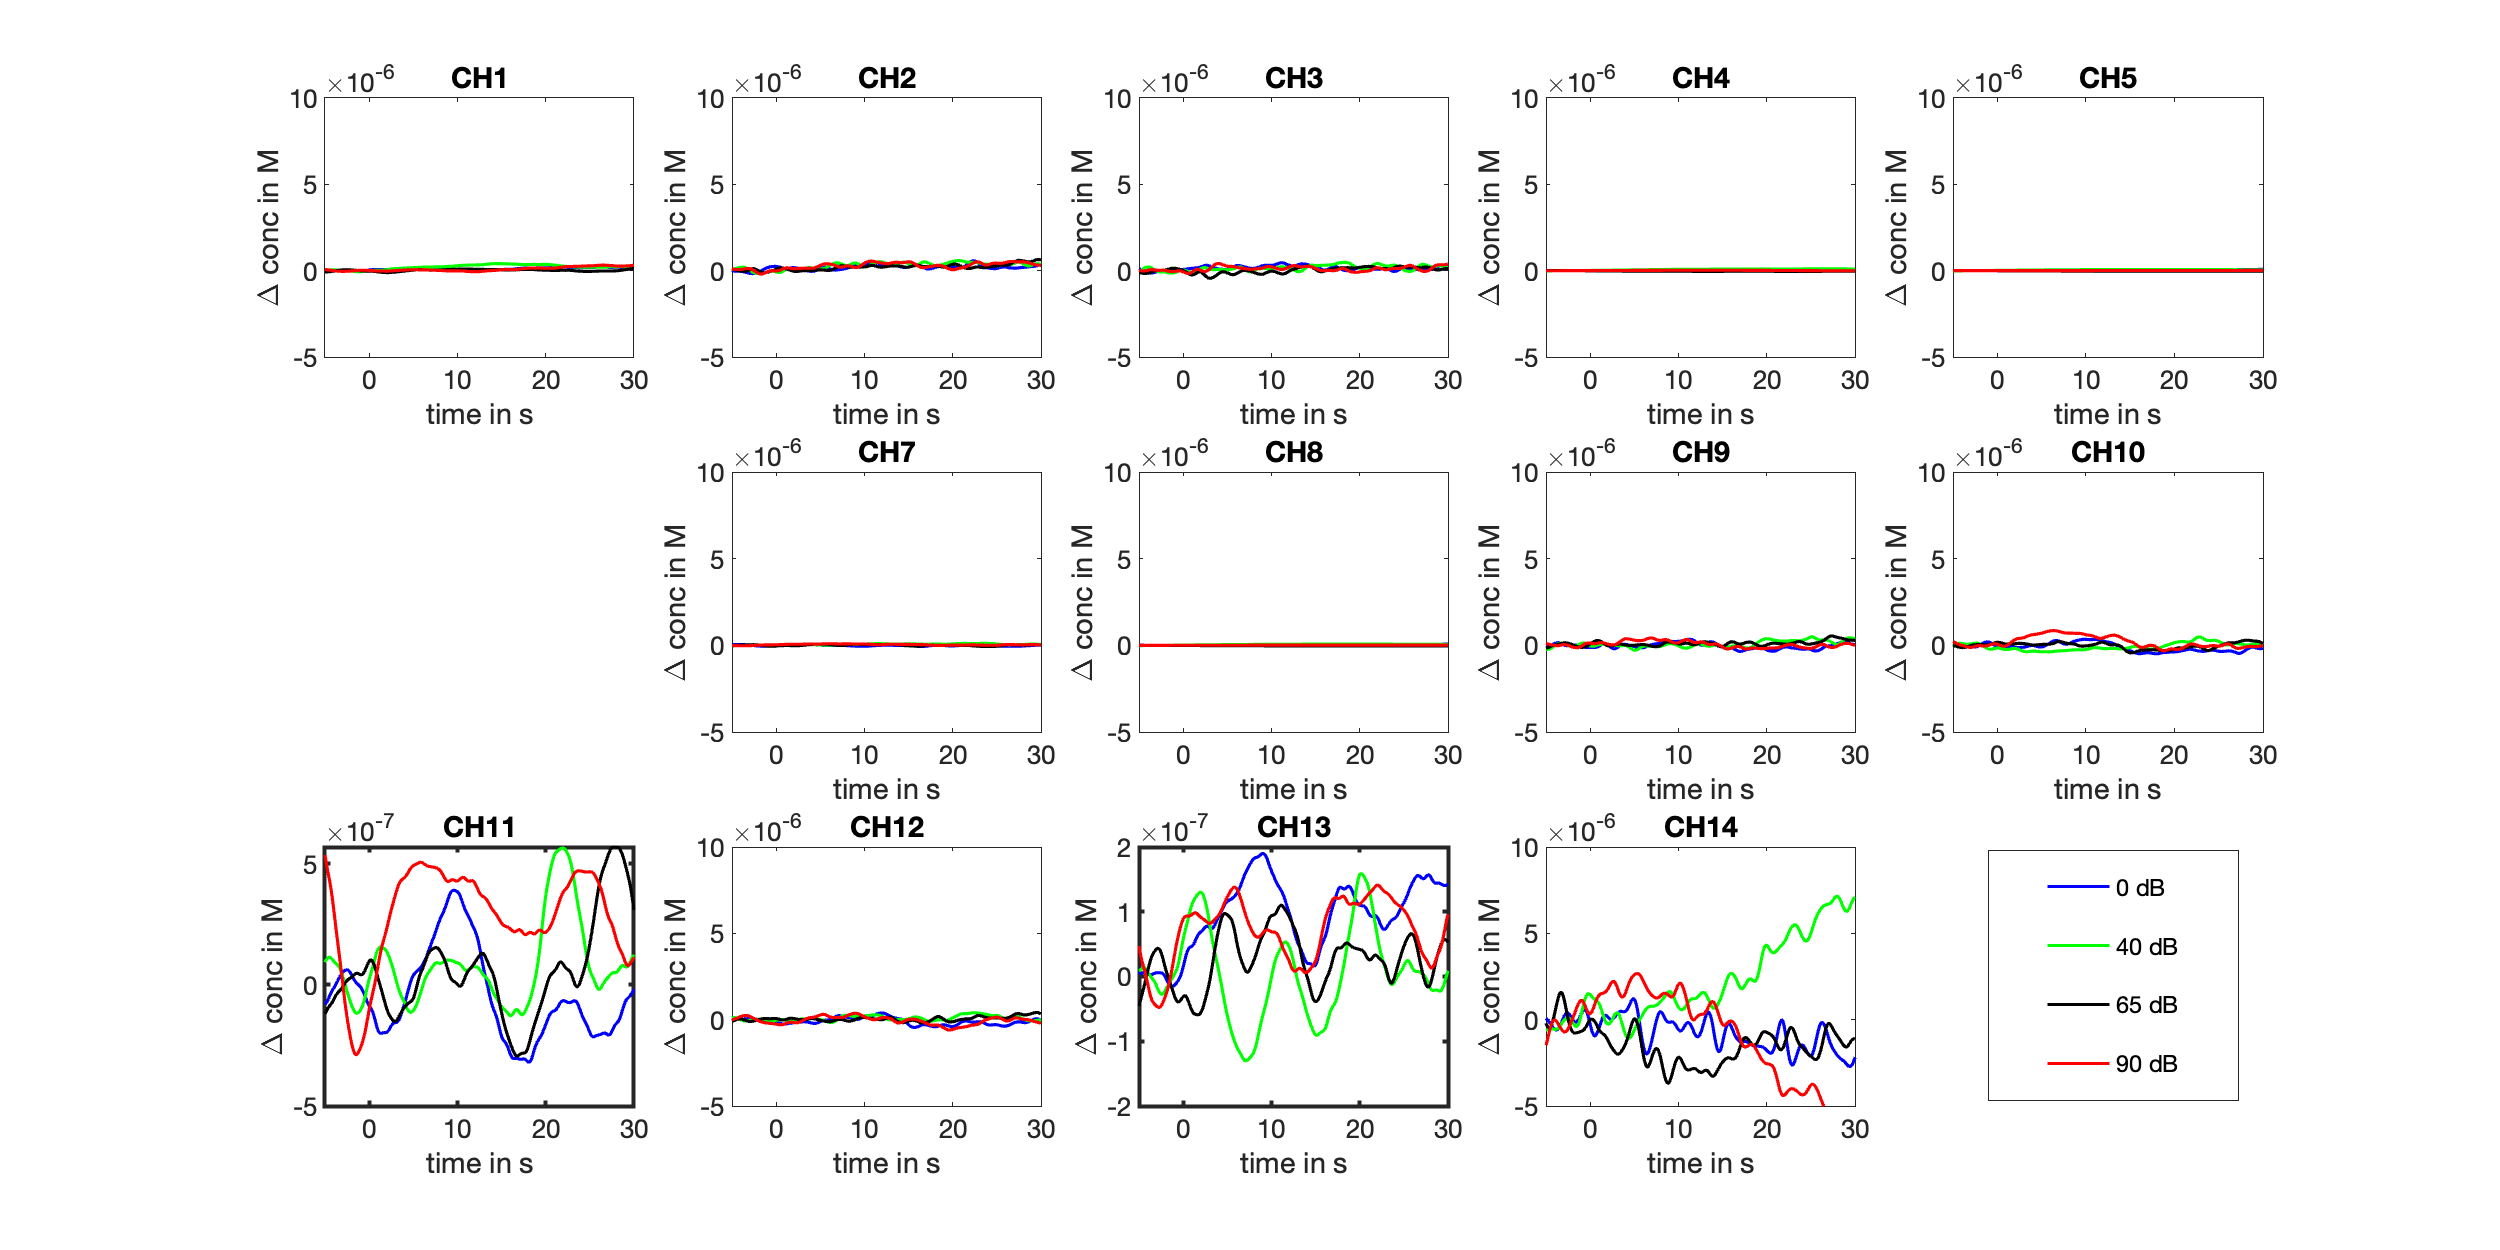
\includegraphics[scale=.35]{bilder/HbO_Mole/sub_lin_s_HbO.png}
  \caption{HbO Measurement from participant 4.}
\end{figure}


\begin{figure}[H]
  \centering
    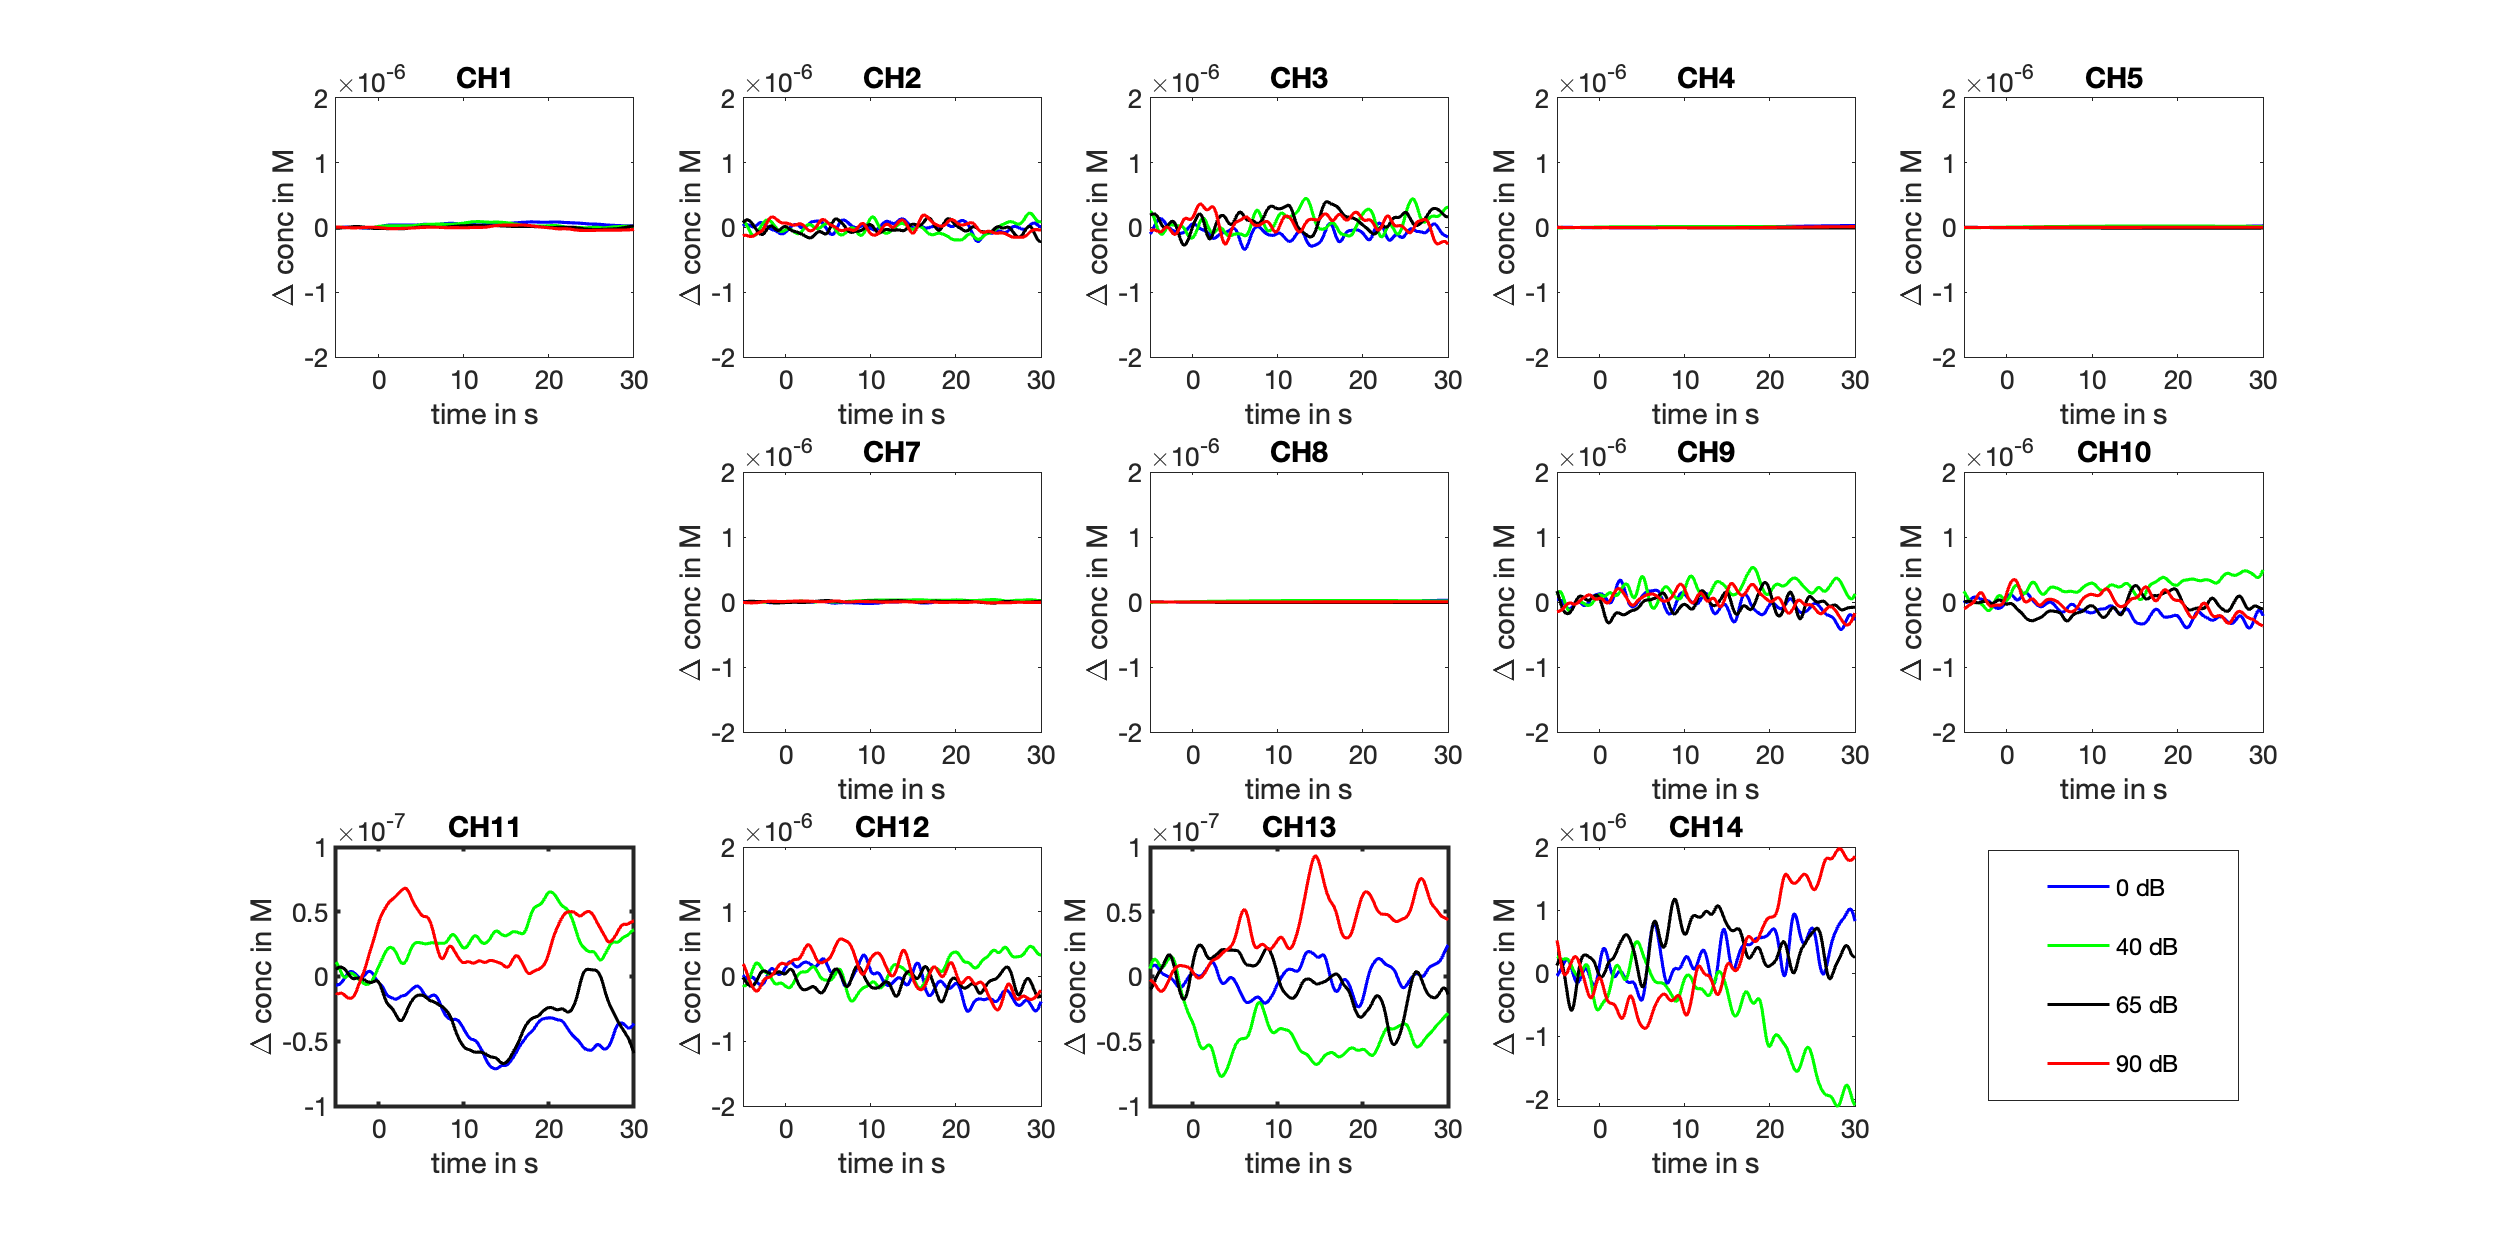
\includegraphics[scale=.35]{bilder/HbR_Mole/sub_lin_s_HbR.png}
  \caption{HbR Measurement from participant 4.}
\end{figure}

\begin{figure}[H]
  \centering
    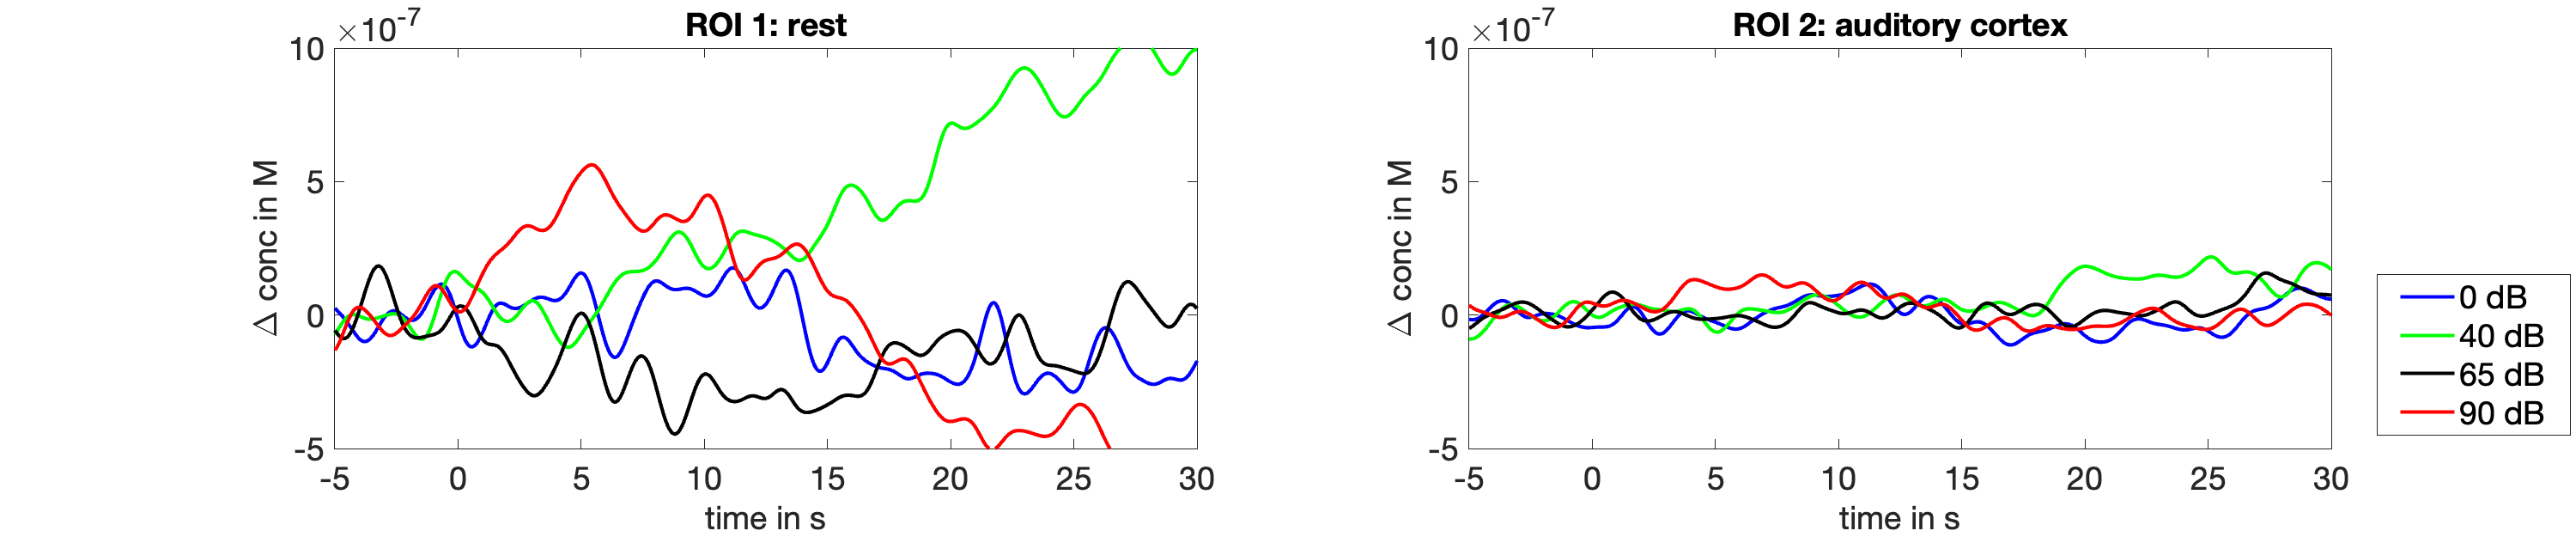
\includegraphics[scale=.29]{bilder/ROI/sub_lin_s_HbO.png}
  \caption{Measurement from participant  4.}
\end{figure}

\newpage



\section {Participant 8}

\begin{figure}[H]
  \centering
    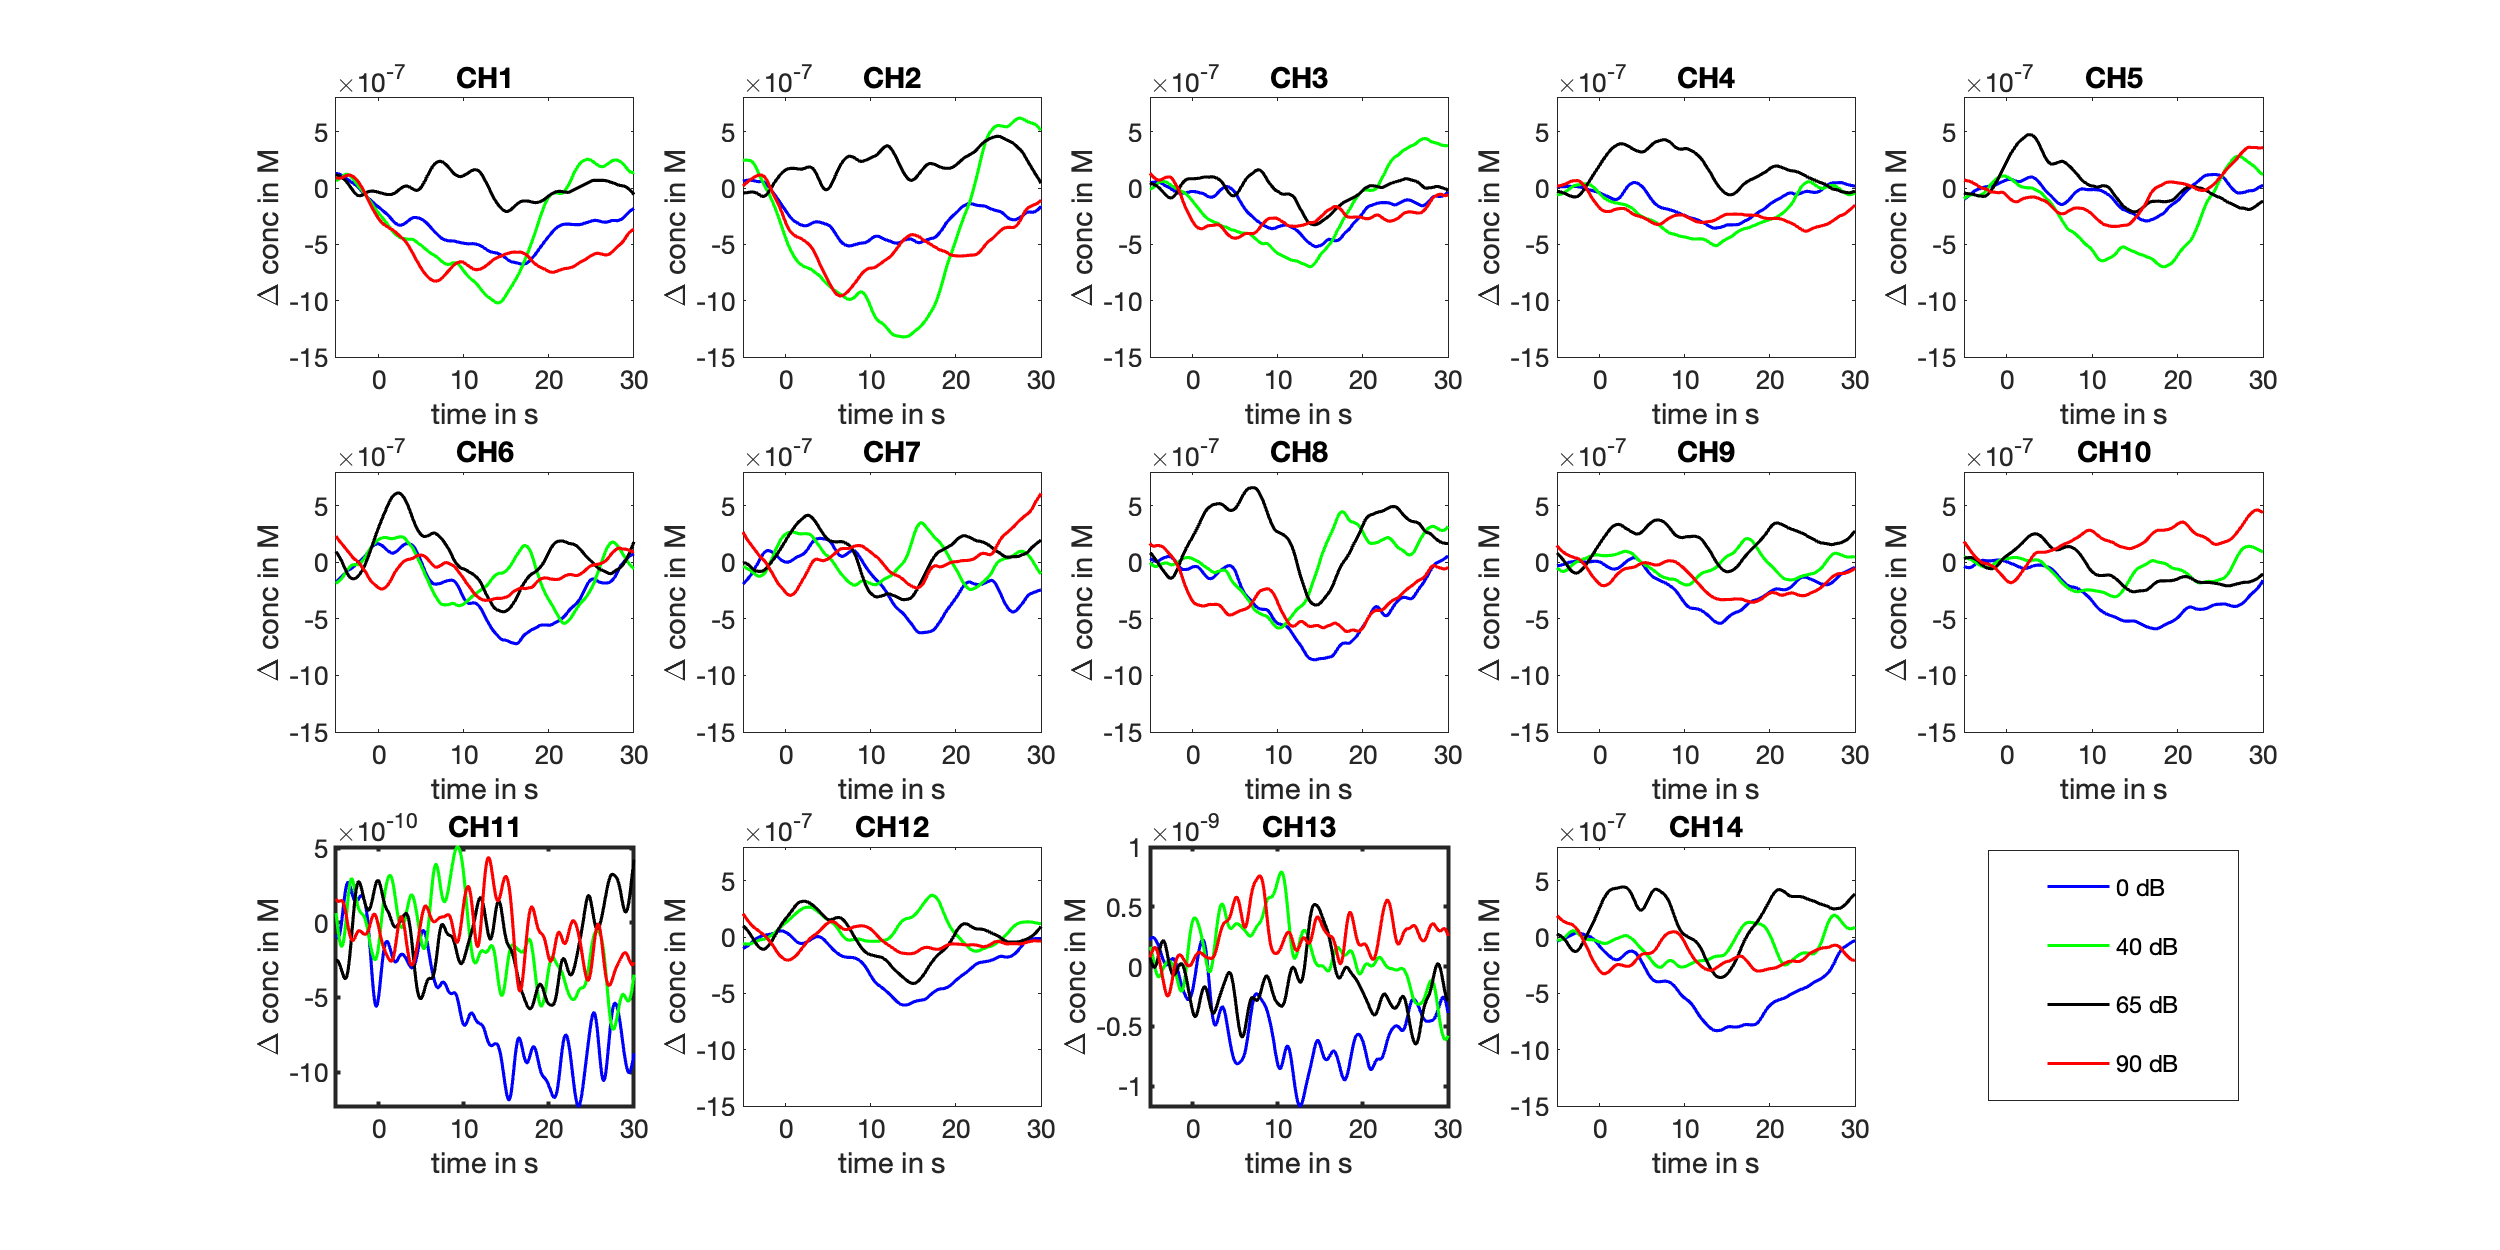
\includegraphics[scale=.4]{bilder/HbO_Mole/sub_luca2_s_HbO.png}
  \caption{Measurement from participant 8. Silent comparison}
  \label{fig:somesignal}
\end{figure}

\begin{figure}[H]
  \centering
    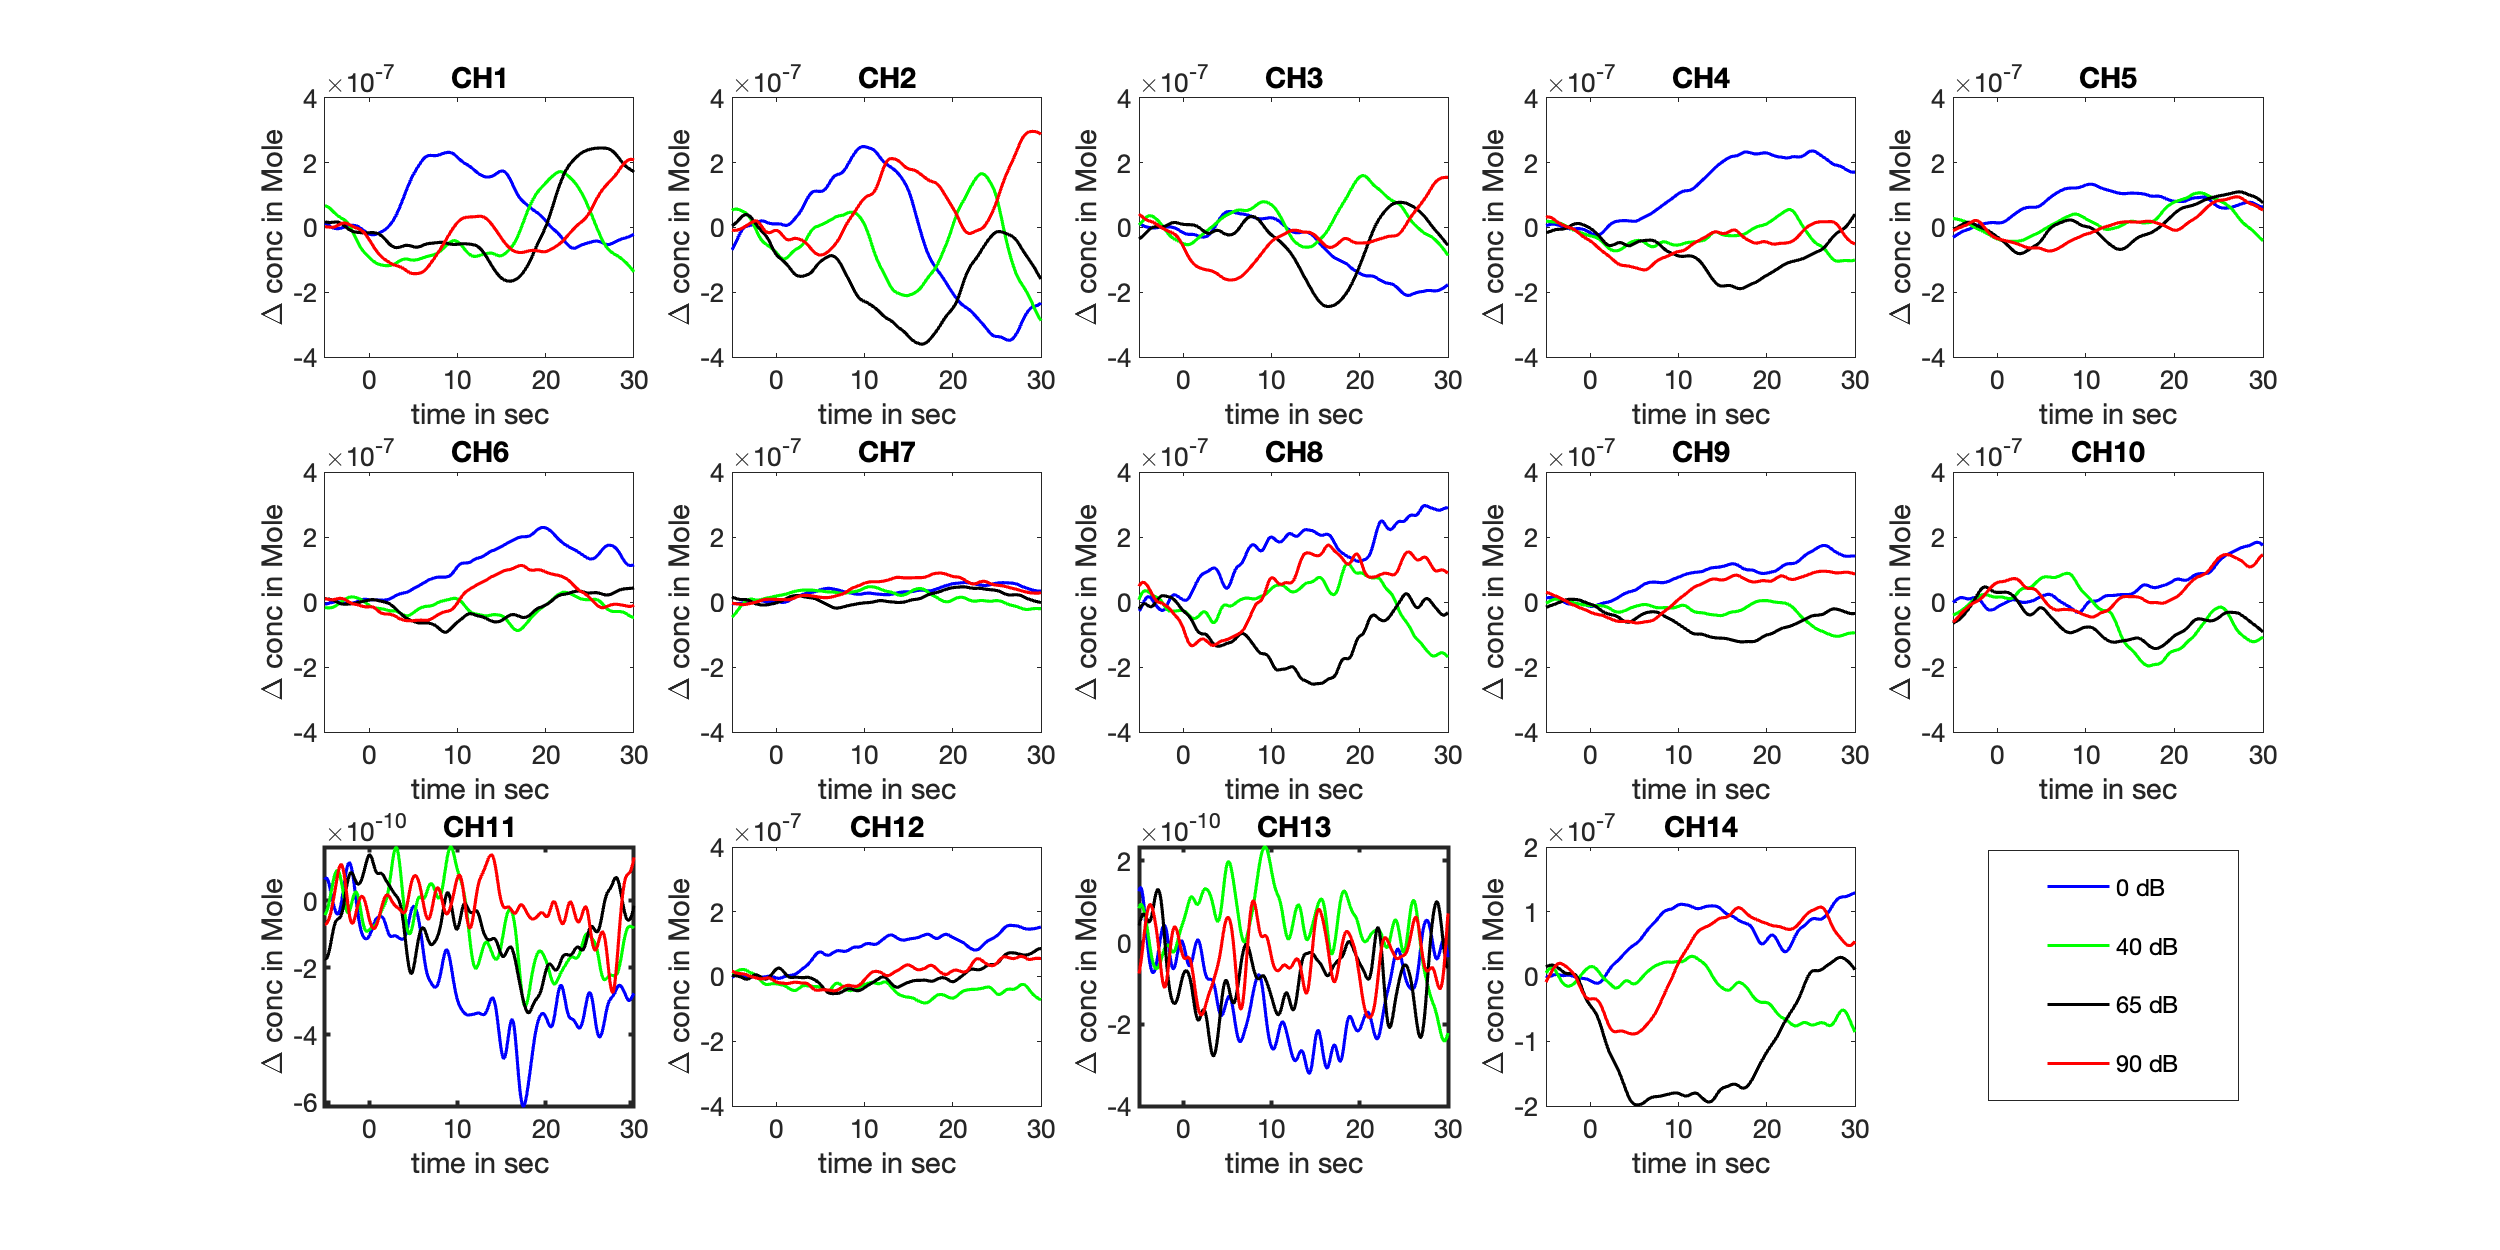
\includegraphics[scale=.4]{bilder/HbR_Mole/sub_luca2_s_HbR.png}
  \caption{Measurement from participant 8. Silent comparison}
\end{figure}

\begin{figure}[H]
  \centering
    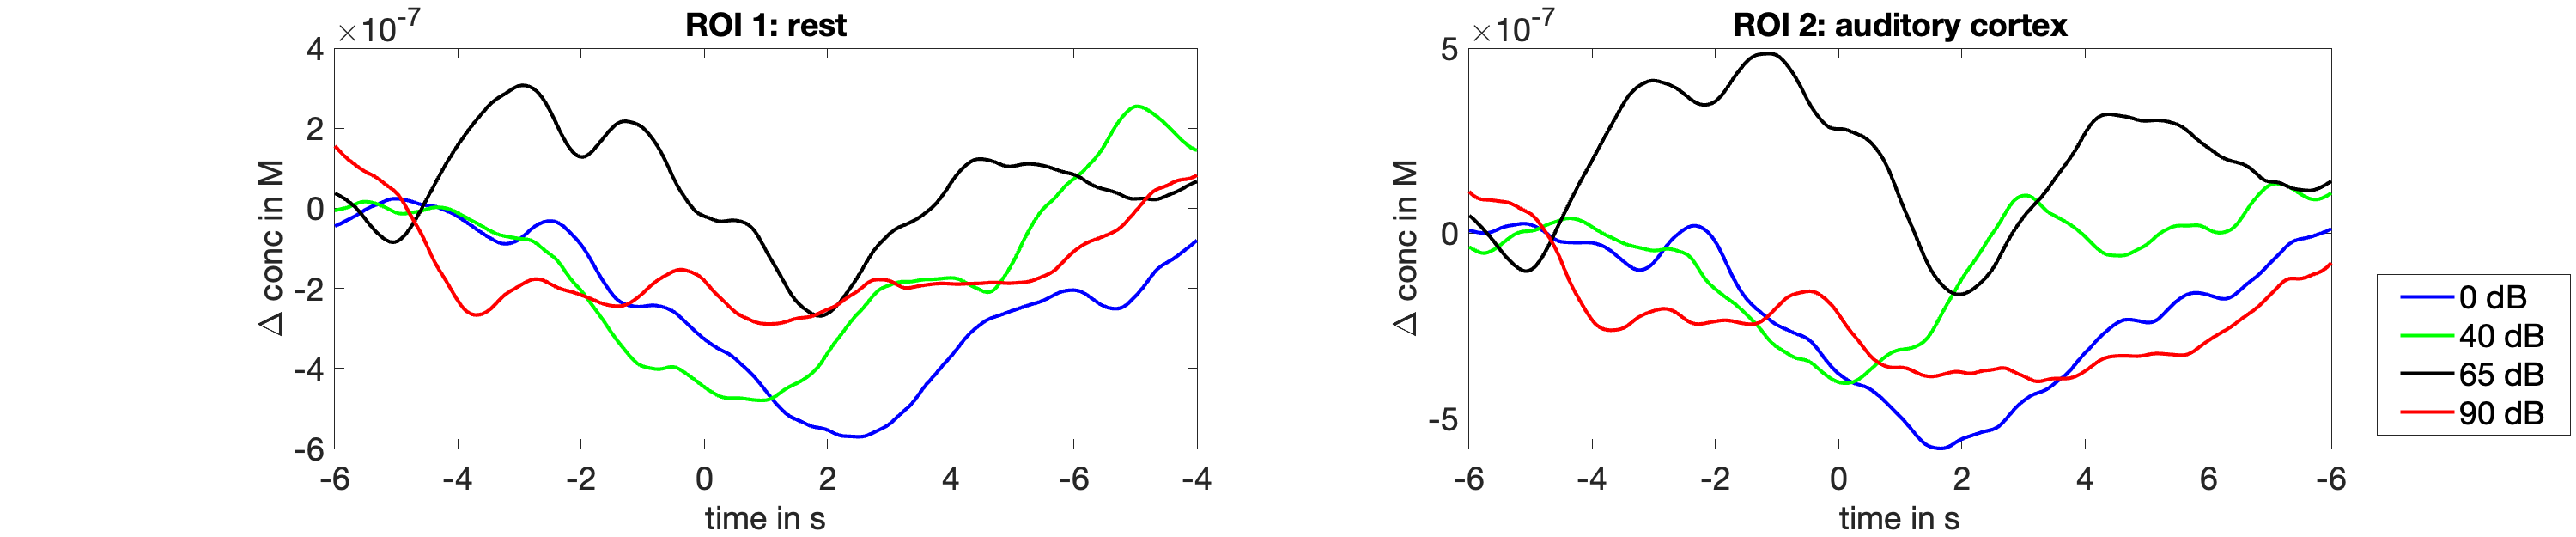
\includegraphics[scale=.29]{bilder/ROI/sub_luca2_s_HbO.png}
  \caption{Measurement from participant 8. Silent comparision.}
\end{figure}

This participant was given only silence stimuli. No pattern could be concluded for the measured waveform morphology. Nonetheless, it's noteworthy to know that even if there are almost no visual and sound stimuli, dynamic hemoglobin response still exists.


%The following plots shows the averaged \textbf {HbO} response of all the valid channels in the defined region.

